% Plantilla para un Trabajo Fin de Grado de la Universidad de Granada,
% adaptada para el Doble Grado en Ingeniería Informática y Matemáticas.
%
%  Autor: Mario Román.
%  Licencia: GNU GPLv2.
%
% Esta plantilla es una adaptación al castellano de la plantilla
% classicthesis de André Miede, que puede obtenerse en:
%  https://ctan.org/tex-archive/macros/latex/contrib/classicthesis?lang=en
% La plantilla original se licencia en GNU GPLv2.
%
% Esta plantilla usa símbolos de la Universidad de Granada sujetos a la normativa
% de identidad visual corporativa, que puede encontrarse en:
% http://secretariageneral.ugr.es/pages/ivc/normativa
%
% La compilación se realiza con las siguientes instrucciones:
%   pdflatex --shell-escape main.tex
%   bibtex main
%   pdflatex --shell-escape main.tex
%   pdflatex --shell-escape main.tex

% Opciones del tipo de documento
\documentclass[oneside,openright,titlepage,numbers=noenddot,openany,headinclude,footinclude=true,
cleardoublepage=empty,abstractoff,BCOR=5mm,paper=a4,fontsize=12pt,main=spanish]{scrreprt}

% Paquetes de latex que se cargan al inicio. Cubren la entrada de
% texto, gráficos, código fuente y símbolofs.
\usepackage[utf8]{inputenc}
\usepackage[T1]{fontenc}
\usepackage{fixltx2e}
\usepackage{graphicx} % Inclusión de imágenes.
\usepackage{grffile}  % Distintos formatos para imágenes.
\usepackage{longtable} % Tablas multipágina.
\usepackage{wrapfig} % Coloca texto alrededor de una figura.
\usepackage{rotating}
\usepackage[normalem]{ulem}
\usepackage{amsmath}
\usepackage{dsfont}
\usepackage{textcomp}
\usepackage{amssymb}
\usepackage{capt-of}
\usepackage[colorlinks=true]{hyperref}
\usepackage{tikz} % Diagramas conmutativos.
\usepackage{minted} % Código fuente.
\usepackage[numbers]{natbib}
\usepackage{booktabs} % Para tablas de figuras (ejemplo en salesman)
\usepackage{listings} % Código

% Plantilla classicthesis
\usepackage[beramono,eulerchapternumbers,linedheaders,parts,a5paper,dottedtoc,
manychapters,pdfspacing]{classicthesis}

% Geometría y espaciado de párrafos.
\setcounter{secnumdepth}{0}
\usepackage{enumitem}
\setitemize{noitemsep,topsep=0pt,parsep=0pt,partopsep=0pt}
\setlist[enumerate]{topsep=0pt,itemsep=-1ex,partopsep=1ex,parsep=1ex}
\usepackage[top=1in, bottom=1.5in, left=1in, right=1in]{geometry}
\setlength\itemsep{0em}
\setlength{\parindent}{0pt}
\usepackage{parskip}

% Profundidad de la tabla de contenidos.
\setcounter{secnumdepth}{3}

% Usa el paquete minted para mostrar trozos de código.
% Pueden seleccionarse el lenguaje apropiado y el estilo del código.
\usepackage{minted}
\usemintedstyle{colorful}
\setminted{fontsize=\small}
\setminted[haskell]{linenos=false,fontsize=\small}
\renewcommand{\theFancyVerbLine}{\sffamily\textcolor[rgb]{0.5,0.5,1.0}{\oldstylenums{\arabic{FancyVerbLine}}}}

% Path para las imágenes
\graphicspath{{figures/}}

% Archivos de configuración.
%------------------------
% Bibliotecas para matemáticas de latex
%------------------------
\usepackage{amsthm}
\usepackage{amsmath}
\usepackage{tikz}
\usepackage{tikz-cd}
\usetikzlibrary{shapes,fit}
\usepackage{bussproofs}
\EnableBpAbbreviations{}
\usepackage{mathtools}
\usepackage{scalerel}
\usepackage{stmaryrd}


%------------------------
% Estilos para los teoremas
%------------------------
\theoremstyle{plain}
\newtheorem{theorem}{Teorema}
\newtheorem{proposition}{Proposición}
\newtheorem{lemma}{Lema}
\newtheorem{corollary}{Corolario}

\theoremstyle{definition}
\newtheorem{definition}{Definición}

% Change the proof style so it's in English and add \qed at the end.
\renewenvironment{proof}{{\bfseries Demostración.}}{\qed}

\theoremstyle{remark}
\newtheorem{remark}{Observación}
\newtheorem{exampleth}{Ejemplo}

% New style for postulates so they are tabulated
\makeatletter
\newtheoremstyle{indented}
	{3pt}% space before
	{3pt}% space after
	{\addtolength{\@totalleftmargin}{3.5em}
		\addtolength{\linewidth}{-3.5em}
		\parshape 1 3.5em \linewidth}% body font
	{}% indent
	{\bfseries}% header font
	{.}% punctuation
	{.5em}% after theorem header
	{}% header specification (empty for default)
\makeatother

% Apply the new style
\theoremstyle{indented}
\newtheorem{postulate}{Postulate}
\newtheorem*{postulate 3'}{Postulate 3'}
\newtheorem*{postulate 2'}{Projective Measurement}

%------------------------
% Macros
% ------------------------

\newcommand*{\B}{\mathbb{B}}
\newcommand*{\C}{\mathds{C}}
\newcommand*{\R}{\mathbb{R}}
\newcommand*{\ra}{\rangle}
\newcommand*{\la}{\langle}

% Para poner sonrisa sobre puntos suspensivos. Uso: \overplace{n}{\dotsc}
\newcommand{\overplace}[2]{%
	\overset{\substack{#1\\\smile}}{#2}%
}

% Para añadir un salto de línea al nuevo párrafo. Use: \newparagraph
\newcommand{\newparagraph}[1]{\paragraph{#1}\mbox{}\\}  % En macros.tex se almacenan las opciones y comandos para escribir matemáticas.
% ****************************************************************************************************
% classicthesis-config.tex 
% formerly known as loadpackages.sty, classicthesis-ldpkg.sty, and classicthesis-preamble.sty 
% Use it at the beginning of your ClassicThesis.tex, or as a LaTeX Preamble 
% in your ClassicThesis.{tex,lyx} with % ****************************************************************************************************
% classicthesis-config.tex 
% formerly known as loadpackages.sty, classicthesis-ldpkg.sty, and classicthesis-preamble.sty 
% Use it at the beginning of your ClassicThesis.tex, or as a LaTeX Preamble 
% in your ClassicThesis.{tex,lyx} with % ****************************************************************************************************
% classicthesis-config.tex 
% formerly known as loadpackages.sty, classicthesis-ldpkg.sty, and classicthesis-preamble.sty 
% Use it at the beginning of your ClassicThesis.tex, or as a LaTeX Preamble 
% in your ClassicThesis.{tex,lyx} with \input{classicthesis-config}
% ****************************************************************************************************  
% If you like the classicthesis, then I would appreciate a postcard. 
% My address can be found in the file ClassicThesis.pdf. A collection 
% of the postcards I received so far is available online at 
% http://postcards.miede.de
% ****************************************************************************************************


% ****************************************************************************************************
% 0. Set the encoding of your files. UTF-8 is the only sensible encoding nowadays. If you can't read
% äöüßáéçèê∂åëæƒÏ€ then change the encoding setting in your editor, not the line below. If your editor
% does not support utf8 use another editor!
% ****************************************************************************************************
\PassOptionsToPackage{utf8x}{inputenc}
	\usepackage{inputenc}

% ****************************************************************************************************
% 1. Configure classicthesis for your needs here, e.g., remove "drafting" below 
% in order to deactivate the time-stamp on the pages
% ****************************************************************************************************
\PassOptionsToPackage{eulerchapternumbers,listings,drafting,%
		pdfspacing,%floatperchapter,%linedheaders,%
                subfig,beramono,eulermath,parts,dottedtoc}{classicthesis}                                        
% ********************************************************************
% Available options for classicthesis.sty 
% (see ClassicThesis.pdf for more information):
% drafting
% parts nochapters linedheaders
% eulerchapternumbers beramono eulermath pdfspacing minionprospacing
% tocaligned dottedtoc manychapters
% listings floatperchapter subfig
% ********************************************************************

% ****************************************************************************************************
% 2. Personal data and user ad-hoc commands
% ****************************************************************************************************
\newcommand{\myTitle}{A Classic Thesis Style\xspace}
\newcommand{\mySubtitle}{An Homage to The Elements of Typographic Style\xspace}
\newcommand{\myDegree}{Doktor-Ingenieur (Dr.-Ing.)\xspace}
\newcommand{\myName}{André Miede\xspace}
\newcommand{\myProf}{Put name here\xspace}
\newcommand{\myOtherProf}{Put name here\xspace}
\newcommand{\mySupervisor}{Put name here\xspace}
\newcommand{\myFaculty}{Put data here\xspace}
\newcommand{\myDepartment}{Put data here\xspace}
\newcommand{\myUni}{Put data here\xspace}
\newcommand{\myLocation}{Saarbrücken\xspace}
\newcommand{\myTime}{September 2015\xspace}
%\newcommand{\myVersion}{version 4.2\xspace}

% ********************************************************************
% Setup, finetuning, and useful commands
% ********************************************************************
\newcounter{dummy} % necessary for correct hyperlinks (to index, bib, etc.)
\newlength{\abcd} % for ab..z string length calculation
\providecommand{\mLyX}{L\kern-.1667em\lower.25em\hbox{Y}\kern-.125emX\@}
\newcommand{\ie}{i.\,e.}
\newcommand{\Ie}{I.\,e.}
\newcommand{\eg}{e.\,g.}
\newcommand{\Eg}{E.\,g.} 
% ****************************************************************************************************


% ****************************************************************************************************
% 3. Loading some handy packages
% ****************************************************************************************************
% ******************************************************************** 
% Packages with options that might require adjustments
% ******************************************************************** 
%\PassOptionsToPackage{ngerman,american}{babel}   % change this to your language(s)
% Spanish languages need extra options in order to work with this template
% \PassOptionsToPackage{es-lcroman,spanish}{babel}
\usepackage[main=spanish]{babel}


%\usepackage{csquotes}
% \PassOptionsToPackage{%
%     %backend=biber, %instead of bibtex
% 	backend=bibtex8,bibencoding=ascii,%
% 	language=auto,%
% 	style=alpha,%
%     %style=authoryear-comp, % Author 1999, 2010
%     %bibstyle=authoryear,dashed=false, % dashed: substitute rep. author with ---
%     sorting=nyt, % name, year, title
%     maxbibnames=10, % default: 3, et al.
%     %backref=true,%
%     natbib=true % natbib compatibility mode (\citep and \citet still work)
% }{biblatex}
%     \usepackage{biblatex}

% \PassOptionsToPackage{fleqn}{amsmath}       % math environments and more by the AMS 
%     \usepackage{amsmath}

% ******************************************************************** 
% General useful packages
% ******************************************************************** 
\PassOptionsToPackage{T1}{fontenc} % T2A for cyrillics
    \usepackage{fontenc}     
\usepackage{textcomp} % fix warning with missing font shapes
\usepackage{scrhack} % fix warnings when using KOMA with listings package          
\usepackage{xspace} % to get the spacing after macros right  
\usepackage{mparhack} % get marginpar right
\usepackage{fixltx2e} % fixes some LaTeX stuff --> since 2015 in the LaTeX kernel (see below)
%\usepackage[latest]{latexrelease} % will be used once available in more distributions (ISSUE #107)
\PassOptionsToPackage{printonlyused,smaller}{acronym} 
    \usepackage{acronym} % nice macros for handling all acronyms in the thesis
    %\renewcommand{\bflabel}[1]{{#1}\hfill} % fix the list of acronyms --> no longer working
    %\renewcommand*{\acsfont}[1]{\textsc{#1}} 
    \renewcommand*{\aclabelfont}[1]{\acsfont{#1}}
% ****************************************************************************************************


% ****************************************************************************************************
% 4. Setup floats: tables, (sub)figures, and captions
% ****************************************************************************************************
\usepackage{tabularx} % better tables
    \setlength{\extrarowheight}{3pt} % increase table row height
\newcommand{\tableheadline}[1]{\multicolumn{1}{c}{\spacedlowsmallcaps{#1}}}
\newcommand{\myfloatalign}{\centering} % to be used with each float for alignment
\usepackage{caption}
% Thanks to cgnieder and Claus Lahiri
% http://tex.stackexchange.com/questions/69349/spacedlowsmallcaps-in-caption-label
% [REMOVED DUE TO OTHER PROBLEMS, SEE ISSUE #82]    
%\DeclareCaptionLabelFormat{smallcaps}{\bothIfFirst{#1}{~}\MakeTextLowercase{\textsc{#2}}}
%\captionsetup{font=small,labelformat=smallcaps} % format=hang,
\captionsetup{font=small} % format=hang,
\usepackage{subfig}  
% ****************************************************************************************************


% ****************************************************************************************************
% 5. Setup code listings
% ****************************************************************************************************
% \usepackage{listings} 
% %\lstset{emph={trueIndex,root},emphstyle=\color{BlueViolet}}%\underbar} % for special keywords
% \lstset{language={Haskell},morekeywords={PassOptionsToPackage,selectlanguage},keywordstyle=\color{RoyalBlue},basicstyle=\small\ttfamily,commentstyle=\color{Green}\ttfamily,stringstyle=\rmfamily,numbers=none,numberstyle=\scriptsize,stepnumber=5,numbersep=8pt,showstringspaces=false,breaklines=true,belowcaptionskip=.75\baselineskip} 
% ****************************************************************************************************             


% ****************************************************************************************************
% 6. PDFLaTeX, hyperreferences and citation backreferences
% ****************************************************************************************************
% ********************************************************************
% Using PDFLaTeX
% ********************************************************************
\PassOptionsToPackage{pdftex,hyperfootnotes=false,pdfpagelabels}{hyperref}
    \usepackage{hyperref}  % backref linktocpage pagebackref
\pdfcompresslevel=9
\pdfadjustspacing=1 
\PassOptionsToPackage{pdftex}{graphicx}
    \usepackage{graphicx} 
 

% ********************************************************************
% Hyperreferences
% ********************************************************************
\hypersetup{%
    %draft, % = no hyperlinking at all (useful in b/w printouts)
    colorlinks=true, linktocpage=true, pdfstartpage=3, pdfstartview=FitV,%
    % uncomment the following line if you want to have black links (e.g., for printing)
    %colorlinks=false, linktocpage=false, pdfstartpage=3, pdfstartview=FitV, pdfborder={0 0 0},%
    breaklinks=true, pdfpagemode=UseNone, pageanchor=true, pdfpagemode=UseOutlines,%
    plainpages=false, bookmarksnumbered, bookmarksopen=true, bookmarksopenlevel=1,%
    hypertexnames=true, pdfhighlight=/O,%nesting=true,%frenchlinks,%
    urlcolor=webbrown, linkcolor=RoyalBlue, citecolor=webgreen, %pagecolor=RoyalBlue,%
    %urlcolor=Black, linkcolor=Black, citecolor=Black, %pagecolor=Black,%
    pdftitle={\myTitle},%
    pdfauthor={\textcopyright\ \myName, \myUni, \myFaculty},%
    pdfsubject={},%
    pdfkeywords={},%
    pdfcreator={pdfLaTeX},%
    pdfproducer={LaTeX with hyperref and classicthesis}%
}   

% ********************************************************************
% Setup autoreferences
% ********************************************************************
% There are some issues regarding autorefnames
% http://www.ureader.de/msg/136221647.aspx
% http://www.tex.ac.uk/cgi-bin/texfaq2html?label=latexwords
% you have to redefine the makros for the 
% language you use, e.g., american, ngerman
% (as chosen when loading babel/AtBeginDocument)
% ********************************************************************
\makeatletter
\@ifpackageloaded{babel}%
    {%
        
       \addto\extrasamerican{%
			\renewcommand*{\figureautorefname}{Figure}%
			\renewcommand*{\tableautorefname}{Table}%
			\renewcommand*{\partautorefname}{Part}%
			\renewcommand*{\chapterautorefname}{Chapter}%
			\renewcommand*{\sectionautorefname}{Section}%
			\renewcommand*{\subsectionautorefname}{Section}%
			\renewcommand*{\subsubsectionautorefname}{Section}%     
                }%
       \addto\extrasngerman{% 
			\renewcommand*{\paragraphautorefname}{Absatz}%
			\renewcommand*{\subparagraphautorefname}{Unterabsatz}%
			\renewcommand*{\footnoteautorefname}{Fu\"snote}%
			\renewcommand*{\FancyVerbLineautorefname}{Zeile}%
			\renewcommand*{\theoremautorefname}{Theorem}%
			\renewcommand*{\appendixautorefname}{Anhang}%
			\renewcommand*{\equationautorefname}{Gleichung}%        
			\renewcommand*{\itemautorefname}{Punkt}%
                }%  
            % Fix to getting autorefs for subfigures right (thanks to Belinda Vogt for changing the definition)
            \providecommand{\subfigureautorefname}{\figureautorefname}%             
    }{\relax}
\makeatother


% ****************************************************************************************************
% 7. Last calls before the bar closes
% ****************************************************************************************************
% ********************************************************************
% Development Stuff
% ********************************************************************
\listfiles
%\PassOptionsToPackage{l2tabu,orthodox,abort}{nag}
%   \usepackage{nag}
%\PassOptionsToPackage{warning, all}{onlyamsmath}
%   \usepackage{onlyamsmath}

% ********************************************************************
% Last, but not least...
% ********************************************************************
\usepackage{classicthesis} 
% ****************************************************************************************************


% ****************************************************************************************************
% 8. Further adjustments (experimental)
% ****************************************************************************************************
% ********************************************************************
% Changing the text area
% ********************************************************************
%\linespread{1.05} % a bit more for Palatino
%\areaset[current]{312pt}{761pt} % 686 (factor 2.2) + 33 head + 42 head \the\footskip
%\setlength{\marginparwidth}{7em}%
%\setlength{\marginparsep}{2em}%

% ********************************************************************
% Using different fonts
% ********************************************************************
%\usepackage[oldstylenums]{kpfonts} % oldstyle notextcomp
%\usepackage[osf]{libertine}
%\usepackage[light,condensed,math]{iwona}
%\renewcommand{\sfdefault}{iwona}
%\usepackage{lmodern} % <-- no osf support :-(
%\usepackage{cfr-lm} % 
%\usepackage[urw-garamond]{mathdesign} <-- no osf support :-(
%\usepackage[default,osfigures]{opensans} % scale=0.95 
%\usepackage[sfdefault]{FiraSans}
% ****************************************************************************************************
% ****************************************************************************************************  
% If you like the classicthesis, then I would appreciate a postcard. 
% My address can be found in the file ClassicThesis.pdf. A collection 
% of the postcards I received so far is available online at 
% http://postcards.miede.de
% ****************************************************************************************************


% ****************************************************************************************************
% 0. Set the encoding of your files. UTF-8 is the only sensible encoding nowadays. If you can't read
% äöüßáéçèê∂åëæƒÏ€ then change the encoding setting in your editor, not the line below. If your editor
% does not support utf8 use another editor!
% ****************************************************************************************************
\PassOptionsToPackage{utf8x}{inputenc}
	\usepackage{inputenc}

% ****************************************************************************************************
% 1. Configure classicthesis for your needs here, e.g., remove "drafting" below 
% in order to deactivate the time-stamp on the pages
% ****************************************************************************************************
\PassOptionsToPackage{eulerchapternumbers,listings,drafting,%
		pdfspacing,%floatperchapter,%linedheaders,%
                subfig,beramono,eulermath,parts,dottedtoc}{classicthesis}                                        
% ********************************************************************
% Available options for classicthesis.sty 
% (see ClassicThesis.pdf for more information):
% drafting
% parts nochapters linedheaders
% eulerchapternumbers beramono eulermath pdfspacing minionprospacing
% tocaligned dottedtoc manychapters
% listings floatperchapter subfig
% ********************************************************************

% ****************************************************************************************************
% 2. Personal data and user ad-hoc commands
% ****************************************************************************************************
\newcommand{\myTitle}{A Classic Thesis Style\xspace}
\newcommand{\mySubtitle}{An Homage to The Elements of Typographic Style\xspace}
\newcommand{\myDegree}{Doktor-Ingenieur (Dr.-Ing.)\xspace}
\newcommand{\myName}{André Miede\xspace}
\newcommand{\myProf}{Put name here\xspace}
\newcommand{\myOtherProf}{Put name here\xspace}
\newcommand{\mySupervisor}{Put name here\xspace}
\newcommand{\myFaculty}{Put data here\xspace}
\newcommand{\myDepartment}{Put data here\xspace}
\newcommand{\myUni}{Put data here\xspace}
\newcommand{\myLocation}{Saarbrücken\xspace}
\newcommand{\myTime}{September 2015\xspace}
%\newcommand{\myVersion}{version 4.2\xspace}

% ********************************************************************
% Setup, finetuning, and useful commands
% ********************************************************************
\newcounter{dummy} % necessary for correct hyperlinks (to index, bib, etc.)
\newlength{\abcd} % for ab..z string length calculation
\providecommand{\mLyX}{L\kern-.1667em\lower.25em\hbox{Y}\kern-.125emX\@}
\newcommand{\ie}{i.\,e.}
\newcommand{\Ie}{I.\,e.}
\newcommand{\eg}{e.\,g.}
\newcommand{\Eg}{E.\,g.} 
% ****************************************************************************************************


% ****************************************************************************************************
% 3. Loading some handy packages
% ****************************************************************************************************
% ******************************************************************** 
% Packages with options that might require adjustments
% ******************************************************************** 
%\PassOptionsToPackage{ngerman,american}{babel}   % change this to your language(s)
% Spanish languages need extra options in order to work with this template
% \PassOptionsToPackage{es-lcroman,spanish}{babel}
\usepackage[main=spanish]{babel}


%\usepackage{csquotes}
% \PassOptionsToPackage{%
%     %backend=biber, %instead of bibtex
% 	backend=bibtex8,bibencoding=ascii,%
% 	language=auto,%
% 	style=alpha,%
%     %style=authoryear-comp, % Author 1999, 2010
%     %bibstyle=authoryear,dashed=false, % dashed: substitute rep. author with ---
%     sorting=nyt, % name, year, title
%     maxbibnames=10, % default: 3, et al.
%     %backref=true,%
%     natbib=true % natbib compatibility mode (\citep and \citet still work)
% }{biblatex}
%     \usepackage{biblatex}

% \PassOptionsToPackage{fleqn}{amsmath}       % math environments and more by the AMS 
%     \usepackage{amsmath}

% ******************************************************************** 
% General useful packages
% ******************************************************************** 
\PassOptionsToPackage{T1}{fontenc} % T2A for cyrillics
    \usepackage{fontenc}     
\usepackage{textcomp} % fix warning with missing font shapes
\usepackage{scrhack} % fix warnings when using KOMA with listings package          
\usepackage{xspace} % to get the spacing after macros right  
\usepackage{mparhack} % get marginpar right
\usepackage{fixltx2e} % fixes some LaTeX stuff --> since 2015 in the LaTeX kernel (see below)
%\usepackage[latest]{latexrelease} % will be used once available in more distributions (ISSUE #107)
\PassOptionsToPackage{printonlyused,smaller}{acronym} 
    \usepackage{acronym} % nice macros for handling all acronyms in the thesis
    %\renewcommand{\bflabel}[1]{{#1}\hfill} % fix the list of acronyms --> no longer working
    %\renewcommand*{\acsfont}[1]{\textsc{#1}} 
    \renewcommand*{\aclabelfont}[1]{\acsfont{#1}}
% ****************************************************************************************************


% ****************************************************************************************************
% 4. Setup floats: tables, (sub)figures, and captions
% ****************************************************************************************************
\usepackage{tabularx} % better tables
    \setlength{\extrarowheight}{3pt} % increase table row height
\newcommand{\tableheadline}[1]{\multicolumn{1}{c}{\spacedlowsmallcaps{#1}}}
\newcommand{\myfloatalign}{\centering} % to be used with each float for alignment
\usepackage{caption}
% Thanks to cgnieder and Claus Lahiri
% http://tex.stackexchange.com/questions/69349/spacedlowsmallcaps-in-caption-label
% [REMOVED DUE TO OTHER PROBLEMS, SEE ISSUE #82]    
%\DeclareCaptionLabelFormat{smallcaps}{\bothIfFirst{#1}{~}\MakeTextLowercase{\textsc{#2}}}
%\captionsetup{font=small,labelformat=smallcaps} % format=hang,
\captionsetup{font=small} % format=hang,
\usepackage{subfig}  
% ****************************************************************************************************


% ****************************************************************************************************
% 5. Setup code listings
% ****************************************************************************************************
% \usepackage{listings} 
% %\lstset{emph={trueIndex,root},emphstyle=\color{BlueViolet}}%\underbar} % for special keywords
% \lstset{language={Haskell},morekeywords={PassOptionsToPackage,selectlanguage},keywordstyle=\color{RoyalBlue},basicstyle=\small\ttfamily,commentstyle=\color{Green}\ttfamily,stringstyle=\rmfamily,numbers=none,numberstyle=\scriptsize,stepnumber=5,numbersep=8pt,showstringspaces=false,breaklines=true,belowcaptionskip=.75\baselineskip} 
% ****************************************************************************************************             


% ****************************************************************************************************
% 6. PDFLaTeX, hyperreferences and citation backreferences
% ****************************************************************************************************
% ********************************************************************
% Using PDFLaTeX
% ********************************************************************
\PassOptionsToPackage{pdftex,hyperfootnotes=false,pdfpagelabels}{hyperref}
    \usepackage{hyperref}  % backref linktocpage pagebackref
\pdfcompresslevel=9
\pdfadjustspacing=1 
\PassOptionsToPackage{pdftex}{graphicx}
    \usepackage{graphicx} 
 

% ********************************************************************
% Hyperreferences
% ********************************************************************
\hypersetup{%
    %draft, % = no hyperlinking at all (useful in b/w printouts)
    colorlinks=true, linktocpage=true, pdfstartpage=3, pdfstartview=FitV,%
    % uncomment the following line if you want to have black links (e.g., for printing)
    %colorlinks=false, linktocpage=false, pdfstartpage=3, pdfstartview=FitV, pdfborder={0 0 0},%
    breaklinks=true, pdfpagemode=UseNone, pageanchor=true, pdfpagemode=UseOutlines,%
    plainpages=false, bookmarksnumbered, bookmarksopen=true, bookmarksopenlevel=1,%
    hypertexnames=true, pdfhighlight=/O,%nesting=true,%frenchlinks,%
    urlcolor=webbrown, linkcolor=RoyalBlue, citecolor=webgreen, %pagecolor=RoyalBlue,%
    %urlcolor=Black, linkcolor=Black, citecolor=Black, %pagecolor=Black,%
    pdftitle={\myTitle},%
    pdfauthor={\textcopyright\ \myName, \myUni, \myFaculty},%
    pdfsubject={},%
    pdfkeywords={},%
    pdfcreator={pdfLaTeX},%
    pdfproducer={LaTeX with hyperref and classicthesis}%
}   

% ********************************************************************
% Setup autoreferences
% ********************************************************************
% There are some issues regarding autorefnames
% http://www.ureader.de/msg/136221647.aspx
% http://www.tex.ac.uk/cgi-bin/texfaq2html?label=latexwords
% you have to redefine the makros for the 
% language you use, e.g., american, ngerman
% (as chosen when loading babel/AtBeginDocument)
% ********************************************************************
\makeatletter
\@ifpackageloaded{babel}%
    {%
        
       \addto\extrasamerican{%
			\renewcommand*{\figureautorefname}{Figure}%
			\renewcommand*{\tableautorefname}{Table}%
			\renewcommand*{\partautorefname}{Part}%
			\renewcommand*{\chapterautorefname}{Chapter}%
			\renewcommand*{\sectionautorefname}{Section}%
			\renewcommand*{\subsectionautorefname}{Section}%
			\renewcommand*{\subsubsectionautorefname}{Section}%     
                }%
       \addto\extrasngerman{% 
			\renewcommand*{\paragraphautorefname}{Absatz}%
			\renewcommand*{\subparagraphautorefname}{Unterabsatz}%
			\renewcommand*{\footnoteautorefname}{Fu\"snote}%
			\renewcommand*{\FancyVerbLineautorefname}{Zeile}%
			\renewcommand*{\theoremautorefname}{Theorem}%
			\renewcommand*{\appendixautorefname}{Anhang}%
			\renewcommand*{\equationautorefname}{Gleichung}%        
			\renewcommand*{\itemautorefname}{Punkt}%
                }%  
            % Fix to getting autorefs for subfigures right (thanks to Belinda Vogt for changing the definition)
            \providecommand{\subfigureautorefname}{\figureautorefname}%             
    }{\relax}
\makeatother


% ****************************************************************************************************
% 7. Last calls before the bar closes
% ****************************************************************************************************
% ********************************************************************
% Development Stuff
% ********************************************************************
\listfiles
%\PassOptionsToPackage{l2tabu,orthodox,abort}{nag}
%   \usepackage{nag}
%\PassOptionsToPackage{warning, all}{onlyamsmath}
%   \usepackage{onlyamsmath}

% ********************************************************************
% Last, but not least...
% ********************************************************************
\usepackage{classicthesis} 
% ****************************************************************************************************


% ****************************************************************************************************
% 8. Further adjustments (experimental)
% ****************************************************************************************************
% ********************************************************************
% Changing the text area
% ********************************************************************
%\linespread{1.05} % a bit more for Palatino
%\areaset[current]{312pt}{761pt} % 686 (factor 2.2) + 33 head + 42 head \the\footskip
%\setlength{\marginparwidth}{7em}%
%\setlength{\marginparsep}{2em}%

% ********************************************************************
% Using different fonts
% ********************************************************************
%\usepackage[oldstylenums]{kpfonts} % oldstyle notextcomp
%\usepackage[osf]{libertine}
%\usepackage[light,condensed,math]{iwona}
%\renewcommand{\sfdefault}{iwona}
%\usepackage{lmodern} % <-- no osf support :-(
%\usepackage{cfr-lm} % 
%\usepackage[urw-garamond]{mathdesign} <-- no osf support :-(
%\usepackage[default,osfigures]{opensans} % scale=0.95 
%\usepackage[sfdefault]{FiraSans}
% ****************************************************************************************************
% ****************************************************************************************************  
% If you like the classicthesis, then I would appreciate a postcard. 
% My address can be found in the file ClassicThesis.pdf. A collection 
% of the postcards I received so far is available online at 
% http://postcards.miede.de
% ****************************************************************************************************


% ****************************************************************************************************
% 0. Set the encoding of your files. UTF-8 is the only sensible encoding nowadays. If you can't read
% äöüßáéçèê∂åëæƒÏ€ then change the encoding setting in your editor, not the line below. If your editor
% does not support utf8 use another editor!
% ****************************************************************************************************
\PassOptionsToPackage{utf8x}{inputenc}
	\usepackage{inputenc}

% ****************************************************************************************************
% 1. Configure classicthesis for your needs here, e.g., remove "drafting" below 
% in order to deactivate the time-stamp on the pages
% ****************************************************************************************************
\PassOptionsToPackage{eulerchapternumbers,listings,drafting,%
		pdfspacing,%floatperchapter,%linedheaders,%
                subfig,beramono,eulermath,parts,dottedtoc}{classicthesis}                                        
% ********************************************************************
% Available options for classicthesis.sty 
% (see ClassicThesis.pdf for more information):
% drafting
% parts nochapters linedheaders
% eulerchapternumbers beramono eulermath pdfspacing minionprospacing
% tocaligned dottedtoc manychapters
% listings floatperchapter subfig
% ********************************************************************

% ****************************************************************************************************
% 2. Personal data and user ad-hoc commands
% ****************************************************************************************************
\newcommand{\myTitle}{A Classic Thesis Style\xspace}
\newcommand{\mySubtitle}{An Homage to The Elements of Typographic Style\xspace}
\newcommand{\myDegree}{Doktor-Ingenieur (Dr.-Ing.)\xspace}
\newcommand{\myName}{André Miede\xspace}
\newcommand{\myProf}{Put name here\xspace}
\newcommand{\myOtherProf}{Put name here\xspace}
\newcommand{\mySupervisor}{Put name here\xspace}
\newcommand{\myFaculty}{Put data here\xspace}
\newcommand{\myDepartment}{Put data here\xspace}
\newcommand{\myUni}{Put data here\xspace}
\newcommand{\myLocation}{Saarbrücken\xspace}
\newcommand{\myTime}{September 2015\xspace}
%\newcommand{\myVersion}{version 4.2\xspace}

% ********************************************************************
% Setup, finetuning, and useful commands
% ********************************************************************
\newcounter{dummy} % necessary for correct hyperlinks (to index, bib, etc.)
\newlength{\abcd} % for ab..z string length calculation
\providecommand{\mLyX}{L\kern-.1667em\lower.25em\hbox{Y}\kern-.125emX\@}
\newcommand{\ie}{i.\,e.}
\newcommand{\Ie}{I.\,e.}
\newcommand{\eg}{e.\,g.}
\newcommand{\Eg}{E.\,g.} 
% ****************************************************************************************************


% ****************************************************************************************************
% 3. Loading some handy packages
% ****************************************************************************************************
% ******************************************************************** 
% Packages with options that might require adjustments
% ******************************************************************** 
%\PassOptionsToPackage{ngerman,american}{babel}   % change this to your language(s)
% Spanish languages need extra options in order to work with this template
% \PassOptionsToPackage{es-lcroman,spanish}{babel}
\usepackage[main=spanish]{babel}


%\usepackage{csquotes}
% \PassOptionsToPackage{%
%     %backend=biber, %instead of bibtex
% 	backend=bibtex8,bibencoding=ascii,%
% 	language=auto,%
% 	style=alpha,%
%     %style=authoryear-comp, % Author 1999, 2010
%     %bibstyle=authoryear,dashed=false, % dashed: substitute rep. author with ---
%     sorting=nyt, % name, year, title
%     maxbibnames=10, % default: 3, et al.
%     %backref=true,%
%     natbib=true % natbib compatibility mode (\citep and \citet still work)
% }{biblatex}
%     \usepackage{biblatex}

% \PassOptionsToPackage{fleqn}{amsmath}       % math environments and more by the AMS 
%     \usepackage{amsmath}

% ******************************************************************** 
% General useful packages
% ******************************************************************** 
\PassOptionsToPackage{T1}{fontenc} % T2A for cyrillics
    \usepackage{fontenc}     
\usepackage{textcomp} % fix warning with missing font shapes
\usepackage{scrhack} % fix warnings when using KOMA with listings package          
\usepackage{xspace} % to get the spacing after macros right  
\usepackage{mparhack} % get marginpar right
\usepackage{fixltx2e} % fixes some LaTeX stuff --> since 2015 in the LaTeX kernel (see below)
%\usepackage[latest]{latexrelease} % will be used once available in more distributions (ISSUE #107)
\PassOptionsToPackage{printonlyused,smaller}{acronym} 
    \usepackage{acronym} % nice macros for handling all acronyms in the thesis
    %\renewcommand{\bflabel}[1]{{#1}\hfill} % fix the list of acronyms --> no longer working
    %\renewcommand*{\acsfont}[1]{\textsc{#1}} 
    \renewcommand*{\aclabelfont}[1]{\acsfont{#1}}
% ****************************************************************************************************


% ****************************************************************************************************
% 4. Setup floats: tables, (sub)figures, and captions
% ****************************************************************************************************
\usepackage{tabularx} % better tables
    \setlength{\extrarowheight}{3pt} % increase table row height
\newcommand{\tableheadline}[1]{\multicolumn{1}{c}{\spacedlowsmallcaps{#1}}}
\newcommand{\myfloatalign}{\centering} % to be used with each float for alignment
\usepackage{caption}
% Thanks to cgnieder and Claus Lahiri
% http://tex.stackexchange.com/questions/69349/spacedlowsmallcaps-in-caption-label
% [REMOVED DUE TO OTHER PROBLEMS, SEE ISSUE #82]    
%\DeclareCaptionLabelFormat{smallcaps}{\bothIfFirst{#1}{~}\MakeTextLowercase{\textsc{#2}}}
%\captionsetup{font=small,labelformat=smallcaps} % format=hang,
\captionsetup{font=small} % format=hang,
\usepackage{subfig}  
% ****************************************************************************************************


% ****************************************************************************************************
% 5. Setup code listings
% ****************************************************************************************************
% \usepackage{listings} 
% %\lstset{emph={trueIndex,root},emphstyle=\color{BlueViolet}}%\underbar} % for special keywords
% \lstset{language={Haskell},morekeywords={PassOptionsToPackage,selectlanguage},keywordstyle=\color{RoyalBlue},basicstyle=\small\ttfamily,commentstyle=\color{Green}\ttfamily,stringstyle=\rmfamily,numbers=none,numberstyle=\scriptsize,stepnumber=5,numbersep=8pt,showstringspaces=false,breaklines=true,belowcaptionskip=.75\baselineskip} 
% ****************************************************************************************************             


% ****************************************************************************************************
% 6. PDFLaTeX, hyperreferences and citation backreferences
% ****************************************************************************************************
% ********************************************************************
% Using PDFLaTeX
% ********************************************************************
\PassOptionsToPackage{pdftex,hyperfootnotes=false,pdfpagelabels}{hyperref}
    \usepackage{hyperref}  % backref linktocpage pagebackref
\pdfcompresslevel=9
\pdfadjustspacing=1 
\PassOptionsToPackage{pdftex}{graphicx}
    \usepackage{graphicx} 
 

% ********************************************************************
% Hyperreferences
% ********************************************************************
\hypersetup{%
    %draft, % = no hyperlinking at all (useful in b/w printouts)
    colorlinks=true, linktocpage=true, pdfstartpage=3, pdfstartview=FitV,%
    % uncomment the following line if you want to have black links (e.g., for printing)
    %colorlinks=false, linktocpage=false, pdfstartpage=3, pdfstartview=FitV, pdfborder={0 0 0},%
    breaklinks=true, pdfpagemode=UseNone, pageanchor=true, pdfpagemode=UseOutlines,%
    plainpages=false, bookmarksnumbered, bookmarksopen=true, bookmarksopenlevel=1,%
    hypertexnames=true, pdfhighlight=/O,%nesting=true,%frenchlinks,%
    urlcolor=webbrown, linkcolor=RoyalBlue, citecolor=webgreen, %pagecolor=RoyalBlue,%
    %urlcolor=Black, linkcolor=Black, citecolor=Black, %pagecolor=Black,%
    pdftitle={\myTitle},%
    pdfauthor={\textcopyright\ \myName, \myUni, \myFaculty},%
    pdfsubject={},%
    pdfkeywords={},%
    pdfcreator={pdfLaTeX},%
    pdfproducer={LaTeX with hyperref and classicthesis}%
}   

% ********************************************************************
% Setup autoreferences
% ********************************************************************
% There are some issues regarding autorefnames
% http://www.ureader.de/msg/136221647.aspx
% http://www.tex.ac.uk/cgi-bin/texfaq2html?label=latexwords
% you have to redefine the makros for the 
% language you use, e.g., american, ngerman
% (as chosen when loading babel/AtBeginDocument)
% ********************************************************************
\makeatletter
\@ifpackageloaded{babel}%
    {%
        
       \addto\extrasamerican{%
			\renewcommand*{\figureautorefname}{Figure}%
			\renewcommand*{\tableautorefname}{Table}%
			\renewcommand*{\partautorefname}{Part}%
			\renewcommand*{\chapterautorefname}{Chapter}%
			\renewcommand*{\sectionautorefname}{Section}%
			\renewcommand*{\subsectionautorefname}{Section}%
			\renewcommand*{\subsubsectionautorefname}{Section}%     
                }%
       \addto\extrasngerman{% 
			\renewcommand*{\paragraphautorefname}{Absatz}%
			\renewcommand*{\subparagraphautorefname}{Unterabsatz}%
			\renewcommand*{\footnoteautorefname}{Fu\"snote}%
			\renewcommand*{\FancyVerbLineautorefname}{Zeile}%
			\renewcommand*{\theoremautorefname}{Theorem}%
			\renewcommand*{\appendixautorefname}{Anhang}%
			\renewcommand*{\equationautorefname}{Gleichung}%        
			\renewcommand*{\itemautorefname}{Punkt}%
                }%  
            % Fix to getting autorefs for subfigures right (thanks to Belinda Vogt for changing the definition)
            \providecommand{\subfigureautorefname}{\figureautorefname}%             
    }{\relax}
\makeatother


% ****************************************************************************************************
% 7. Last calls before the bar closes
% ****************************************************************************************************
% ********************************************************************
% Development Stuff
% ********************************************************************
\listfiles
%\PassOptionsToPackage{l2tabu,orthodox,abort}{nag}
%   \usepackage{nag}
%\PassOptionsToPackage{warning, all}{onlyamsmath}
%   \usepackage{onlyamsmath}

% ********************************************************************
% Last, but not least...
% ********************************************************************
\usepackage{classicthesis} 
% ****************************************************************************************************


% ****************************************************************************************************
% 8. Further adjustments (experimental)
% ****************************************************************************************************
% ********************************************************************
% Changing the text area
% ********************************************************************
%\linespread{1.05} % a bit more for Palatino
%\areaset[current]{312pt}{761pt} % 686 (factor 2.2) + 33 head + 42 head \the\footskip
%\setlength{\marginparwidth}{7em}%
%\setlength{\marginparsep}{2em}%

% ********************************************************************
% Using different fonts
% ********************************************************************
%\usepackage[oldstylenums]{kpfonts} % oldstyle notextcomp
%\usepackage[osf]{libertine}
%\usepackage[light,condensed,math]{iwona}
%\renewcommand{\sfdefault}{iwona}
%\usepackage{lmodern} % <-- no osf support :-(
%\usepackage{cfr-lm} % 
%\usepackage[urw-garamond]{mathdesign} <-- no osf support :-(
%\usepackage[default,osfigures]{opensans} % scale=0.95 
%\usepackage[sfdefault]{FiraSans}
% **************************************************************************************************** % En classicthesis-config.tex se almacenan las opciones propias de la plantilla.

% Color institucional UGR
% \definecolor{ugrColor}{HTML}{ed1c3e} % Versión clara.
\definecolor{ugrColor}{HTML}{c6474b}  % Usado en el título.
\definecolor{ugrColor2}{HTML}{c6474b} % Usado en las secciones.

% Datos de portada
\usepackage{titling} % Facilita los datos de la portada
\author{Paula Villanueva Núñez} 
\title{Criptoanálisis del Criptosistema \\ de McEliece clásico \\ mediante algoritmos genéticos}

% Portada
\usepackage{datetime}
\renewcommand\maketitle{
  \begin{titlepage}
    \begin{addmargin}[-2.5cm]{-3cm}
      \begin{center}
        \normalsize  
        \hfill
        \vfill
        \vspace{1.8cm}

        \spacedallcaps{TRABAJO FIN DE GRADO} \\ \medskip 
        \small{\spacedallcaps{Doble grado en Ingeniería Informática y Matemáticas}} \\  \bigskip\bigskip
        \vspace{1.5cm}

        \begingroup
        \LARGE{\color{ugrColor}\spacedallcaps{\textbf{\thetitle}}} \\ \bigskip
        \endgroup

        \vfill
        \vspace{1.5cm}

        \textbf{Autora}\\
        \spacedlowsmallcaps{\theauthor}

        \textbf{Director}\\
        \spacedlowsmallcaps{Gabriel Navarro Garulo} \\  \bigskip

        \hfill
        \vspace{1.7cm}

        
\includegraphics[scale=0.18]{figures/fciencias_logo.png} 
        \quad
        
\includegraphics{figures/etsiit_logo.png}


        \spacedlowsmallcaps{Facultad de Ciencias} \\
        \spacedlowsmallcaps{E.T.S. de Ingenierías Informática y de Telecomunicación} \\ \medskip
        \vspace{1.0cm}
        %\textit{Curso académico 2021-2022}
        \textit{Granada, a \today}

        \vfill                      

      \end{center}  
    \end{addmargin}       
  \end{titlepage}}
\usepackage{wallpaper}
\usepackage[main=spanish]{babel}

\begin{document}

\ThisULCornerWallPaper{1}{figures/ugrA4.pdf}
\maketitle

% TODO: dedicatoria
%\newpage

\thispagestyle{empty}
\phantomsection

\hfill
\vfill

\begin{flushright}
	\itshape
	% TODO: poner aquí la dedicatoria
\end{flushright}

\vfill

\endinput
\newpage

% Indice
\tableofcontents

% TODO: Resumen
%\newpage
\null
\thispagestyle{empty}

\chapter*{Resumen}
%\addcontentsline{toc}{chapter}{Resumen} 

La posible existencia de ordenadores cuánticos amenaza la seguridad de los sistemas criptográficos más conocidos y usados en la actualidad, como RSA. En este trabajo se propone, se estudia y se implementa un criptosistema resistente a estos ataques, el criptosistema de McEliece clásico, junto a una variante, el criptosistema de Niederreiter. Ambos sistemas se construyen a partir de los códigos de Goppa, una clase de códigos de corrección de errores lineales que también desarrollaremos e implementaremos. Estos códigos permiten codificar mensajes y decodificarlos mediante un algoritmo eficiente, el algoritmo de Sugiyama. Previamente, introduciremos y presentaremos los conceptos necesarios para poder abordar el objetivo de este trabajo. Por último, se proponen ataques usando algoritmos genéticos para vulnerar la seguridad del criptosistema de McEliece.

\small{\spacedallcaps{Palabras clave:} teoría de códigos, \; Goppa, \; criptografía, \; criptografía post-cuántica, \; McEliece, \; Niederreiter, \; algoritmos genéticos, \; SageMath}

\newpage
%\newpage
\null
\thispagestyle{empty}

\chapter*{Summary}
%\addcontentsline{toc}{chapter}{Summary} 

\begin{otherlanguage}{english}

The main goal of this project is to present, study and implement a cryptosystem resistant to attacks by quantum computers, the McEliece cryptosystem.

\spacedlowsmallcaps{Chapter 1}

In this chapter we will present the previous mathematical concepts necessary to understand the subsequent development of this work. We will need to introduce concepts such as finite fields, since they are the algebraic structure on which we will work. We will also deal with the complexity of algorithms and problems, which will be useful to know if we can obtain a solution in polynomial time. Eventually, we will introduce the basic concepts of population-based metaheuristics to further develop genetic algorithms, which will be useful in attempting to break the security of McEliece's cryptosystem.

\spacedlowsmallcaps{Chapter 2}

In the second chapter we will study linear codes, defined as a subspace of a finite field. We will introduce two concepts that will be of great importance throughout the development of this work: the generating matrix and the parity matrix. Each of these matrices presents a unique code. We will also define some significant measures along with their properties, such as the Hamming distance or the Hamming weight. We will deal with the complexity of the problem of finding a word with minimum weight and related issues. We will finish by presenting the Brouwer-Zimmermann algorithm for calculating the distance of a code.

\spacedlowsmallcaps{Chapter 3}

In this chapter we will develop and implement a new class of linear error correcting codes, the Goppa codes. We will study the parity matrix associated with these codes and we will obtain from it the generating matrix, which will be useful for encoding the messages. We will also analyze the corrective capacity, which will depend on the degree of the polynomial on which the code is defined. In addition, we will develop the encoding and decoding process, including examples of the implementation carried out. For the decoding we will use an efficient algorithm, the Sugiyama algorithm, which is based on the Euclid algorithm and will allow us to recover the messages.

\newpage

\spacedlowsmallcaps{Chapter 4}

The fourth chapter contains the study of the goal of this project, the McEliece cryptosystem. Previously, we will introduce the concept and objectives of cryptography, as well as two main types of cryptosystems. Next, we will present the possibility of the existence of quantum computers and the threat that they present to the security of some existing cryptosystems, proposing some alternatives that are capable of resisting their attacks, such as the McEliece cryptosystem. This system is constructed from the Goppa codes studied in the previous chapter. We will study the generation of its keys (public and private), as well as the encryption and decryption processes. We will also analyze a variant, the Niederreiter system, which is equivalent in security. We will present examples of the McEliece system using the implementation carried out to show its operation.

\spacedlowsmallcaps{Chapter 5}

In this last chapter, we will develop a couple of attacks using genetic algorithms to break the security of McEliece's cryptosystem. These attacks are based on calculating the distance of a code from an echelon matrix of a matrix that generates the equivalent code, which will be obtained by swapping the code columns. We will study and implement adaptations of the GGA and CHC algorithms. Finally, we will analyze the results obtained after applying these algorithms to the McEliece system.

To carry out this project, the following has been implemented in SageMath.

\begin{itemize}
    \item A class to define the Goppa codes, another class for your encoder, and another class for your decoder using Sugiyama's algorithm. The documentation of this class can be found in the annex \ref{annex:sage-Goppa}, along with the helpful functions used.
    \item A class to define the McEliece cryptosystem, whose documentation can be found in the annex \ref{annex:sage-McEliece}, along with the helpful functions used.
    \item One function for the GGA genetic algorithm and another function for the CHC genetic algorithm. The documentation of these functions, along with other helpful functions used, can be found in the annex \ref{annex:sage-geneticos}.
\end{itemize}

\small{\spacedallcaps{Keywords:} coding theory, \; Goppa, \; criptography, \; post-quantum criptography, \; McEliece, \; Niederreiter, \; genetic algorithms, \; SageMath}

\end{otherlanguage}

% TODO: Introducción
%\chapter*{Introducción y objetivos}
\addcontentsline{toc}{chapter}{Introducción y objetivos}

%TODO: poner aquí introducción y objetivos

\textcolor{red}{Añadir introducción y objetivos}


\begin{comment}

La introducción deberá:
- Contextualizar el trabajo explicando antecedentes importantes para el desarrollo realizado y efectuando, en su caso, un estudio de los progresos recientes.
- Describir el problema abordado, de forma que el lector tenga desde este momento una idea clara de la cuestión a resolver o del producto  a desarrollar y una  visión general de la solución alcanzada.
- Exponer con claridad las técnicas y áreas matemáticas, así como los conceptos y herramientas de la ingeniería informática que se han empleado.
- Sintetizar el contenido de la memoria.
- Citar las principales fuentes consultadas.

Objetivos del trabajo:
- En  este apartado deberán aparecer con claridad los objetivos inicialmente previstos en la propuesta de TFG y los finalmente alcanzados con indicación de  dificultades, cambios y mejoras respecto a la propuesta inicial. Si procede, es conveniente apuntar de manera precisalas interdependencias entre los distintos objetivos y conectarlos con los diferentes apartadosde la memoria. 
Se pueden destacar aquí los aspectos formativos previos más utilizados.
\end{comment}



% TODO: Capítulos
% 0. Preliminares. 
% Esto es voluntario. 
% Consiste en poner lo que ya sabías, porque lo has dado en el grado, y que te haga falta 
% (por ejemplo, algebra lineal, cuerpos finitos, operaciones con polinomios, algoritmos genéticos, etc).

\chapter{Preliminares}

En este capítulo se desarrollarán las herramientas necesarias para poder afrontar el criptosistema de McEliece que precisa este trabajo. Empezaremos abordando concepto de anillo y algunas de sus propiedades más importantes. A partir de este noción, podremos definir los cuerpos finitos y los conceptos relacionados con ellos, tales como los anillos de polinomios sobre cuerpos finitos y su utilidad para construir cuerpos finitos. También será de especial relevancia tratar los conceptos relacionados con la teoría de la complejidad para clasificar los problemas de acuerdo a su dificultad. Finalmente, estudiaremos las metaheurísticas basadas en la población para introducir los algoritmos genéticos.

\section{Anillos}

En esta sección introduciremos el concepto de anillo para poder definir el concepto de cuerpo, así como las principales propiedades de esta estructura algebraica.

\begin{definition}
    Un \emph{anillo} $(A, +, \cdot )$ es un conjunto $A$ junto con dos operaciones binarias $A \times A \rightarrow A$ denotadas por la suma (denotada por $+$) y producto (denotado por $\cdot$) que verifican los siguientes axiomas:

    \begin{itemize}
        \item Propiedad asociativa de la suma: 
        $$  a + (b + c) = (a + b) + c \qquad \forall a,b,c \in A$$
        \item Existencia del elemento neutro para la suma:
        $$ 0 + a = a = a + 0 \qquad \forall a \in A$$
        \item Existencia del elemento inverso para la suma:
        $$ \forall a \in A \; \; \exists -a \in A \quad a + (-a) = 0 = (-a) + a $$
        \item Propiedad conmutativa de la suma:
        $$ a + b = b + a \qquad \forall a,b \in A $$
        \item Propiedad asociativa del producto:
        $$ a \cdot (b \cdot c) = (a \cdot b) \cdot c \qquad \forall a,b,c \in A $$
        \item Propiedad distributiva del producto:
        $$ a \cdot (b + c) = a \cdot b + a \cdot c, \quad (b + c) \cdot a = b \cdot a + c \cdot a \qquad \forall a,b,c \in A $$
        
    \end{itemize}

    Un anillo de llama \emph{conmutativo o abeliano} si se verifica la propiedad conmutativa del producto 
    $$ ab = ba \qquad \forall a,b \in A $$
\end{definition}

Es fácil comprobar que en todo anillo se verifica $0 \cdot x = x \cdot 0 = 0$ (obsérvese que $0 \cdot = (0 + 0) \cdot x = 0 \cdot x + 0 \cdot x$ y simplifíquese por el simétrico de $0 \cdot x$).

Además del anillo conmutativo, existen otros casos particulares de anillos. Diremos que un anillo es \emph{unitario} si es un anillo cuyo producto tiene elemento neutro, esto es, $\exists 1 \in A \; : \; x \cdot 1 = 1 \cdot x = x$, para todo $x \in A$.

Diremos que un elemento $a$ del anillo $A$ es \emph{invertible} si existe un elemento $a'$ en el anillo $A$ tal que $a \cdot a' = a' \cdot a = 1$. Este elemento $a'$ es único, lo llamaremos \emph{elemento inverso} y lo denotaremos por $a^{-1}$.

Cuando se da la igualdad $1 = 0$, diremos que el anillo es \emph{trivial} y tendrá un solo elemento.

\begin{definition}
    Sea $A$ un anillo, $1 \in A$ el elemento neutro del producto y $n \geq 1$ un número natural, definimos la cardinalidad de $A$ como:

    \[
        Car(A) = \left\{ \begin{array}{lc}
        0 &   \textit{si } n \cdot 1 \neq 0 \textit{ para cualquier } n \geq 1 \\
        \\ n & \textit{si n es el menor número natural no nulo para el que } n \cdot 1 = 0
        \end{array}
        \right.
    \]
\end{definition}

%TODO
% - Añadir homomorfismo de anillos? (apuntes de álgebra I)
% - Añadir subestructuras de anillos e ideales? (apuntes de álgebra I)
% - Añadir propiedades de los dominios de integridad? (apuntes de álgebra I)

\section{Cuerpos finitos}

Para presentar el concepto de cuerpo finito, necesitaremos definir previamente el concepto de cuerpo junto con algunas de sus propiedades más relevantes.

\begin{definition}
    Un \emph{cuerpo} $(K, +, \cdot)$ es un anillo conmutativo no trivial en el que todo elemento no nulo tiene un inverso multiplicativo. Se dice que un cuerpo es \emph{finito} si tiene un número finito de elementos.
\end{definition}

Sea $(K, +, \cdot)$ un cuerpo y $E \subset K$, diremos que $E$ es un \emph{subcuerpo} de $K$ o $K$ es una \emph{extensión} de $E$ si se cumple que $(E, +, \cdot)$ es un cuerpo cuando las operaciones $+$ y $\cdot$ se restringen a $E$.

Diremos que la \emph{característica} de un cuerpo es el número de elementos que tiene.

Todos los cuerpos finitos tienen un número de elementos $q = p^n$, para algún número primo $p$ y algún entero positivo $n$. Denotaremos por $\mathbb{F}_q$ a los cuerpos finitos con característica $q$, aunque otra común notación es $GF(q)$.

Observemos que si $p$ un número primo y $q$ es un número entero tal que $q = p^n$, entonces $\mathbb{F}_q$ es un espacio vectorial sobre $\mathbb{F}_p$ de dimensión $n$. Además, hay $q$ vectores en el espacio vectorial de dimensión $n$ sobre $\mathbb{F}_p$.

Notemos que todos los cuerpos finitos de orden $q$ son isomorfos, aunque cada cuerpo puede tener diferentes representaciones.

\begin{proposition}
    Sea $\mathbb{F}_q$ un cuerpo finito con $q = p^n$ elementos, entonces 

    $$p \cdot \alpha = 0, \qquad \forall \alpha \in \mathbb{F}_q.$$
\end{proposition}

\begin{proposition}
    Sea $\mathbb{F}_q$ un cuerpo finito con característica $p$, se cumple que

    $$( \alpha + \beta )^p = \alpha^p + \beta^p, \qquad \forall \alpha, \beta \in \mathbb{F}_q.$$
\end{proposition}

% TODO: homomorfismo de cuerpos

\subsection{Anillo de polinomios sobre cuerpos finitos}

En esta sección vamos a introducir el concepto de polinomio junto con sus operaciones.

\begin{definition}
    Sea $A$ un anillo conmutativo. El \emph{conjunto de polinomios} en la variable $x$ con coeficientes en $A$ está compuesto por el siguiente conjunto
    $$\{ a_n x^n  + a_{n-1} x^{n-1} + \cdots + a_1 x + a_0 \; : \; a_0, ..., a_n \in A \}.$$
    Este conjunto se representa por $A[X]$.
\end{definition}

En el conjunto de polinomios definimos una suma y un producto. 

Sean $f = a_n x^n + a_{n-1} x^{n-1} + \cdots + a_1 x + a_0$ y $g = b_m x^m + b_{m-1} x^{m-1} + \cdots + b_1 x + b_0$ dos polinomios. Supongamos que $m \leq n$, tomando $b_i = 0$ para todo $n \geq i > m$, definimos las operaciones de suma y producto de polinomios:

\begin{align*}
    f + g       &= (a_n + b_n)x^n + (a_{n-1} + b_{n-1})x^{n-1} + \cdots + (a_1 + b_1)x + (a_0 + b_0).\\
    f \cdot g   &= a_n b_m x^{n+m} + (a_n b_{m+1} + a_{n-1} b_m) x^{n+m-1} + \cdots + (a_1 b_0 + a_0 b_1)x + a_0 b_0.
\end{align*} 
De esta forma, diremos que el conjunto $A[X]$ con las operaciones anteriores es un \emph{anillo de polinomios en X con coeficientes en A}.

\begin{definition}
    Para un polinomio $f = a_n + a_{n-1} x^{n-1} + \cdots + a_1 x + a_0 \neq 0$ el mayor índice $n$ tal que $a_n \neq 0$ se llama \emph{grado de f} y se representa por $\gr(f)$. Si $f = 0$ definimos $\gr(f) = - \infty$.

    Llamaremos \emph{término (de grado i)} a cada uno de los sumandos $a_i X^i$ del polinomio $f$. El \emph{término líder} es el término no nulo de mayor grado. El coeficiente $a_n \neq 0$ del término líder se llama \emph{coeficiente líder} y el término de grado cero $a_0$ se llama \emph{término constante}. Si el coeficiente líder es $1$, diremos que el polinomio es \emph{mónico}.
\end{definition}

A continuación tenemos algunas propiedades de los polinomios.

\begin{proposition}
    Sea $A$ un anillo conmutativo y sean $f,g \in A[X]$ dos polinomios, tenemos que 
    $$\gr(f + g) \leq \max{(\gr(f), \; \gr(g))},$$
    $$\gr(f \cdot g) \leq \gr(f) + \gr(g)$$
    Si $\gr(f) \neq \gr(g)$, se verifica 
    $$\gr(f + g) = \max{(\gr(f), \; \gr(g))}$$
\end{proposition}

Podemos trasladar estos resultados al caso de los cuerpos finitos. Sea $\mathbb{F}_q$ un cuerpo finito, un polinomio $f(x)$ estará definido sobre dicho cuerpo si es de la forma $f(x) = \sum_{i = 0}^{n} a_i \cdot x^i$, donde $a_i \in \mathbb{F}_q$ para todo $i = 0, ..., n$. Análogamente, diremos que $f(x) \in \mathbb{F}_q$.

Sean $f(x)$ y $g(x)$ polinomios en $\mathbb{F}_q[x]$, diremos que $f(x)$ divide a $g(x)$ si existe un polinomio $h(x) \in \mathbb{F}_q[x]$ tal que $g(x) = f(x) h(x)$ y lo denotaremos por $f(x) \vert g(x)$. El polinomio $f(x)$ se llama \emph{divisor} o \emph{factor} de $g(x)$.

El \emph{mayor común divisor} de $f(x)$ y $g(x)$ es el polinomio mónico en $\mathbb{F}_q[x]$ con mayor grado que divide a $f(x)$ y a $g(x)$. Este polinomio es único y se denota por $\mcd(f(x), \; g(x))$. Diremos que los polinomios $f(x)$ y $g(x)$ son \emph{primos relativos} si $\mcd(f(x), \; g(x)) = 1$.

El siguiente resultado es de gran utilidad, pues sirve para calcular los divisores de un polinomio e incluso para calcular el máximo común divisor. Nos dará las bases para definir posteriormente el Algoritmo de Euclides.

\begin{theorem}
    \label{th:div_alg}
    Sean $f(x)$ y $g(x)$ polinomios en $\mathbb{F}_q[x]$ con $g(x)$ no nulo.
    \begin{itemize}
        \item Existen dos polinomios únicos $c(x), r(x) \in \mathbb{F}_q[x]$ tales que
        $$f(x) = g(x) c(x) + r(x), \qquad \textit{donde } \gr(r(x)) < \gr(g(x)) \textit{ o } r(x) = 0.$$
        \item Si $f(x) = g(x) c(x) + r(x)$, entonces $\mcd(f(x), \; g(x)) = \mcd(g(x), \; r(x))$.
    \end{itemize}
\end{theorem}

Los polinomios $c(x)$ y $r(x)$ se llaman \emph{cociente} y \emph{resto}, respectivamente.

Usando este resultado de forma recursiva, obtendremos el máximo común divisor de los polinomios $f(x)$ y $g(x)$. Este procedimiento se conoce como \emph{Algoritmo de Euclides}. El siguiente resultado describe este algoritmo.

\begin{theorem}[Algoritmo de Euclides]
    \label{th:alg-euclides}
    Sean $f(x)$ y $g(x)$ polinomios definidos en $\mathbb{F}_q[x]$ con $g(x)$ no nulo.
    \begin{enumerate}
        \item Realizar los siguientes pasos hasta que $r_n(x) = 0$ para algún $n$:
            \begin{align*}
                f(x)        &= g(x) c_1(x) + r_1(x), & &\textit{donde } \gr(r_1(x)) < \gr(x),\\
                g(x)        &= r_1(x) c_2(x) + r_2(x),& &\textit{donde } \gr(r_2(x)) < \gr(r_1),\\
                r_1(x)      &= r_2(x) c_3(x) + r_3(x),& &\textit{donde } \gr(r_3(x)) < \gr(r_2),\\
                            &\; \; \vdots & &\\
                r_{n-3}(x)  &= r_{n-2}(x) c_{n-1}(x) + r_{n-1}(x),& &\textit{donde } \gr(r_{n-1}(x)) < \gr(r_{n-2}),\\
                r_{n-2}(x)  &= r_{n-1}(x) c_{n}(x) + r_{n}(x),& &\textit{donde } r_n(x) = 0.
            \end{align*}
            Entonces $\mcd(f(x), \; g(x)) = cr_{n-1}(x)$, donde $c \in \mathbb{F}_q$ es una constante para que $c r_{n-1}(x)$ sea mónico.
        \item Existen polinomios $a(x), b(x) \in \mathbb{F}_q[x]$ tales que 
        $$a(x) f(x) + b(x) g(x) = \mcd(f(x), \; g(x)).$$
    \end{enumerate}
\end{theorem}

En cada paso el grado del resto se decrementa al menos en $1$, por lo que podemos asegurar que la secuencia de pasos anterior terminará en algún momento.

A continuación se muestran algunos resultados relevantes.

\begin{proposition}
    Sean $f(x)$ y $g(x)$ polinomios en $\mathbb{F}_q[x]$.
    \begin{itemize}
        \item Si $k(x)$ es un divisor de $f(x)$ y $g(x)$, entonces $k(x)$ es un divisor de $a(x) f(x) + b(x) g(x)$ para algunos $a(x), b(x) \in \mathbb{F}_q[x]$.
        \item Si $k(x)$ es un divisor de $f(x)$ y $g(x)$, entonces $k(x)$ es un divisor de $\mcd(f(x), \; g(x))$.
    \end{itemize}
\end{proposition}

\begin{proposition}
    Sea $f(x)$ un polinomio en $\mathbb{F}_q[x]$ de grado $n$.
    \begin{itemize}
        \item Si $\alpha \in \mathbb{F}_q$ es una raíz de $f(x)$, entonces $x - \alpha$ es un factor de $f(x)$.
        \item El polinomio $f(x)$ tiene como mucho $n$ raíces en cualquier cuerpo que contenga a $\mathbb{F}_q$.
    \end{itemize}
\end{proposition}

\begin{theorem}
    Los elementos de $\mathbb{F}_q$ son las raíces de $x^q - x$.
\end{theorem}

\subsubsection{Construcción de cuerpos finitos}

Para realizar la construcción de cuerpos finitos, previamente necesitaremos conocer el siguiente concepto y algunos resultados relacionados.

\begin{definition}
    Sea $f(x) \in \mathbb{F}_q[x]$ un polinomio no constante, decimos que es \emph{irreducible} sobre $\mathbb{F}_q$ si no se factoriza como producto de dos polinomios en $\mathbb{F}_q[x]$ de menor grado.
\end{definition}

\begin{theorem}
    Sea $f(x)$ un polinomio no constante. Entonces

    $$f(x) = p_1(x)^{a_1} \cdots p_k(x)^{a_k},$$

    donde cada $p_i(x)$ es irreducible y único salvo orden, y los elementos $a_i$ son únicos.
\end{theorem}

Como consecuencia de este resultado, tenemos que $\mathbb{F}_q[x]$ es un \emph{dominio de factorización única}.

El siguiente resultado nos muestra cómo construir un cuerpo finito de característica $p$ a partir del cociente de anillos de polinomios por polinomios irreducibles.

\begin{proposition}
    Sea $p$ un número primo y sea el polinomio $f(x) \in \mathbb{F}_p[x]$ irreducible en $\mathbb{F}_p$ y de grado $m$. Tenemos que el anillo cociente $\mathbb{F}_q[x]/\left(f(x)\right)$ es un cuerpo finito con $q = p^m$ elementos, es decir, con característica $p$.
\end{proposition}

Escribiremos los elementos del anillo cociente, que son las clases laterales $g(x) + (f(x))$ como vectores en $\mathbb{F}_p^m$ con la siguiente correspondencia:

\begin{equation}
    \label{pr:correspondencia}
    g_{m-1} x^{m-1} + g_{m-2} x^{m-2} + \cdots + g_{1} x + g_0 + (f(x)) \leftrightarrow (g_{m-1}, g_{m-2}, ..., g_1, g_0).
\end{equation}

Esta notación facilita la operación de sumar dos elementos. Sin embargo, la multiplicación es algo más complicada. Supongamos que queremos multiplicar $g_1(x) + (f(x))$ por $g_2(x) + (f(x))$. Para ello, usaremos el resultado \ref{th:div_alg} para obtener

\begin{equation}
    \label{pr:multiplicacion_clase_lateral}
    g_1(x) g_2(x) = f(x) h(x) + r(x),
\end{equation}

donde $\gr(r(x)) \leq m - 1$ o $r(x) = 0$. Entonces 

$$(g_1(x) + (f(x))) (g_2(x) + (f(x))) = r(x) + (f(x)).$$

Podemos simplificar la notación si reemplazamos $x$ por $\alpha$ donde $f(\alpha) = 0$. Por \eqref{pr:multiplicacion_clase_lateral}, se cumple que $g_1(\alpha) g_2(\alpha) = r(\alpha)$ y la correspondencia \eqref{pr:correspondencia} queda como sigue

$$g_{m-1} g_{m-2} \cdots g_1 g_0 \leftrightarrow  g_{m-1} \alpha^{m-1} g_{m-2} \alpha^{m-2}\cdots g_1 \alpha g_0.$$

De esta forma, multiplicamos los polinomios en $\alpha$ de forma usual y aplicamos al resultado que $f(\alpha) = 0$ para reducir las potencias de $\alpha$ mayores que $m-1$ a polinomios en $\alpha$ de grado menor que $m$.


\section{Teoría de la complejidad}

El objetivo de esta sección se basa en clasificar los problemas de acuerdo a su dificultad. Nos centraremos en estudiar la complejidad de los problemas decidibles, es decir, los problemas que pueden tener algoritmos para resolverlos.

\subsection{Complejidad de los algoritmos}

A la hora de resolver un problema con un algoritmo, tendrán gran importancia los recursos que consume dicho algoritmo, sobre todo el espacio y el tiempo. La complejidad del tiempo de un algoritmo es el número de pasos que necesita para resolver un problema de tamaño $n$. La complejidad de un algoritmo siempre se define en el peor de los casos, esto es, se obtiene una cota para el recuento de los pasos en el peor de los casos. 

La siguiente definición nos proporciona la notación más importante en el análisis de los algoritmos.

\begin{definition}[Notación $\mathcal{O}$-grande]
    Sean $f, g : \mathbb{N}^r \longrightarrow \mathbb{R}$. Decimos que $f(n) = O(g(n))$ si existen dos constantes $c \in \mathbb{R}^+$ y $n_0 \in \mathbb{N}^r$ tales que $\forall n \geq n_0$, $f(n) \leq c \cdot g(n)$.
\end{definition}

Con esta notación podemos analizar el tiempo esperado que va a tardar un algoritmo en realizar una tarea.

\begin{proposition}
    Para cualquier $\lambda \in \mathbb{R}^+$ y $g : \mathbb{N}^r \longrightarrow \mathbb{R}$, tenemos que

    $$\mathcal{O}(g(n)) = \mathcal{O}(\lambda g(n)), \qquad \forall n \in \mathbb{N}^r.$$
\end{proposition}

A continuación presentaremos algunos conceptos importantes para especificar la complejidad de los algoritmos que nos serán de utilidad más adelante.

\begin{definition}[Algoritmo en tiempo polinomial]
    Un algoritmo es un \emph{algoritmo en tiempo polinomial} si su complejidad es $\mathcal{O}(p(n))$, donde $p(n)$ es una función polinómica de $n$.
\end{definition}

\begin{definition}[Algoritmo en tiempo exponencial]
    Un algoritmo es un \emph{algoritmo en tiempo exponencial} si su complejidad es $\mathcal{O}(c^n)$, donde $c$ es una constante real estrictamente mayor que $1$.
\end{definition}

\subsection{Complejidad de los problemas}

La complejidad de un problema es equivalente a la complejidad del mejor algoritmo que resuelve ese problema. Diremos que un problema es \emph{fácil} si existe un algoritmo en tiempo polinomial que lo resuelve, mientras que un problema será \emph{difícil} si no existe ningún algoritmo en tiempo polinomial que lo resuelva.

La teoría de la complejidad de los problemas se ocupa de los \emph{problemas de decisión}. Un problema de decisión siempre tiene una respuesta de sí o no.

\begin{figure}[H]   
	\center
	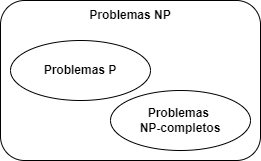
\includegraphics[scale=0.5]{figures/Complejidad.png}
	\caption{Clases de complejidad de los problemas de decisión.}
    \label{fg:complexity}
\end{figure}

Con la teoría computacional podemos clasificar los problemas en sus clases de complejidad. Existen dos clases importantes de problemas: P y NP (Figura \ref{fg:complexity}).

La clase de complejidad P representa a la familia de problemas de decisión que se pueden resolver mediante un algoritmo en tiempo polinomial. Los problemas que pertenecen a esta clase son \emph{fáciles} de resolver.

La clase de compejidad NP representa a la familia de problemas de decisión que se pueden resolver por un algoritmo no determinista en tiempo polinomial. Un algoritmo no determinista tiene algunos puntos en los que hay múltiples combinaciones diferentes sin ninguna especificación de cuál se tomará. Estos problemas se dicen que son más \emph{difíciles} de resolver.

Para definir la clase de los problemas NP-completos, necesitaremos previamente definir el concepto de reducción.

\begin{definition}[Reducción polinómica]
    Un problema de decisión $A$ se \emph{reduce polinómicamente} a otro problema de decisión $B$ si, para todas las instancias de entrada $I_A$ de $A$, siempre se puede construir una instancia de entrada $I_B$ para $B$ en una función de tiempo polinomial, de tal forma que $I_A$ es una instancia positiva de $A$ si y solo si $I_B$ es una instancia positiva de $B$.
\end{definition}

Un problema de decisión es \emph{NP-completo} si es NP y cualquier otro problema de NP se reduce a él. Los problemas que pertenecen a esta clase son los \emph{más difíciles} dentro de la clase NP.

La figura \ref{fg:complexity} muestra la relación entre los problemas P, NP y NP-completos.

Los problemas \emph{NP-duros} son problemas de optimización cuyo problema de decisión asociado es NP-completo. Las metaheurísticas constituyen una importante alternativa para resolver esta clase de problemas.

\section{Metaheurísticas basadas en la población}

Las \emph{metaheurísticas} representan una familia de técnicas de optimización aproximada. Proporcionan soluciones aceptables en un tiempo razonable para resolver problemas difíciles y complejos, esto es, problemas que no pertenecen a la clase de complejidad P o que no se conoce que pertenezcan a dicha clase. Sin embargo, no garantizan la optimalidad de las soluciones obtenidas.

Las \emph{metaheurísticas basadas en la población} se pueden ver como una mejora iterativa en una población de soluciones. Estas metaheurísticas consisten en inicializar la población, posteriormente generan una nueva población de soluciones y finalmente esta nueva población reemplaza a la actual usando algunos procedimientos de selección. Una vez se alcanza la condición dada, el proceso de búsqueda finaliza y obtenemos una solución.

El esquema de este procedimiento se muestra a continuación.

\begin{Ualgorithm}[H]
    \small
    \DontPrintSemicolon
    \KwOut{Mejor solución encontrada}
    $P \longleftarrow P_0$ \tcp{Generación de la población inicial}
    $t \longleftarrow 0$\;
    \While{No se cumpla la condición de parada}{
        Generar($P_t'$) \tcp{Generación de la nueva población}
        $P_{t+1} \longleftarrow $ SeleccionarPoblación($P_t \cup P_t'$) \tcp{Selección de la nueva población}
        $t \longleftarrow t + 1$\;
    }
\end{Ualgorithm}

Vamos a estudiar en detalle este procedimiento concretando los conceptos en los que se basa.

\begin{enumerate}
    \item \textbf{Generación de la población inicial}. Las metaheurísticas basadas en la población comienzan con una población inicial de soluciones. Este paso juega un papel fundamental en la efectividad del algoritmo y su eficiencia. El principal criterio para generar la población es que haya diversidad.
    \item \textbf{Generación de una nueva población}. En este paso, se genera una nueva población de soluciones. Se puede realizar de varias formas, sin embargo la que estudiaremos será la que se basa en la evolución. En esta categoría, las soluciones que componen la población se seleccionan y se reproducen usando operadores de variación (por ejemplo, mutación, recombinación) y actúan directamente sobre sus representaciones. Una nueva solución surge a partir de los diferentes atributos de las soluciones de la población actual.
    \item \textbf{Selección de la nueva población}. Este último paso consiste en seleccionar las nuevas soluciones y reemplazar a la población actual. Este reemplazamiento se puede realizar de varias maneras, por ejemplo una estrategia se basa en seleccionar la nueva población generada como la población actual, otra estrategia se fundamenta en el escoger las dos mejores soluciones de la nueva población y reemplazarlas por las dos peores de la población actual, etc.
\end{enumerate}

El criterio de parada suele ser un número máximo de iteraciones (generaciones), un número máximo de evaluaciones de la función objetivo, etc.

\subsection{Algoritmos evolutivos}

Los \emph{algoritmos evolutivos} son algoritmos basados en poblaciones. Estos se fundamentan en el concepto de \emph{competición}. Se representan como una clase de algoritmos de optimización iterativos que simulan la evolución de las especies, en este caso, la evolución de la población de soluciones.

Inicialmente, tenemos una población de soluciones que suele ser generada aleatoriamente. También tenemos una función objetivo, que es la que queremos optimizar, que evalúa cada individuo perteneciente a la población indicando la idoneidad de pertenencia al problema (\emph{fitness}). En cada paso, los individuos se seleccionan para formar los padres. En esta selección los individuos con mayor fitness tendrán altas probabilidades de ser escogidos. Luego, los individuos seleccionados se reproducen usando operadores de variación (por ejemplo, cruce, mutación) para generar nuevos descendientes, de forma que nos permite explorar el espacio de búsqueda y obtendremos soluciones diversas. Finalmente, el esquema de reemplazamiento se basa en determinar los individuos que sobrevivirán entre los descendientes y los padres. Esta iteración representa una generación. Este proceso es iterativo hasta que se cumpla el criterio de parada.

Cada solución que forma parte de la población se suele llamar \emph{cromosoma}. A su vez, cada cromosoma está formado por \emph{genes}.

\begin{figure}[H]   
	\center
	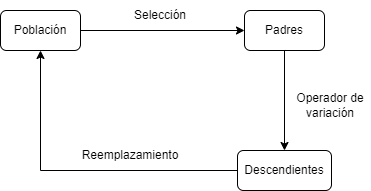
\includegraphics[scale=0.5]{figures/Algoritmos_evolutivos.png}
	\caption{Generación en algoritmos evolutivos.}
    \label{fg:alg_ev}
\end{figure}

El algoritmo \ref{alg:ev} ilustra este procedimiento.

\begin{Ualgorithm}[H]
    \label{alg:ev}
    \small
    \DontPrintSemicolon
    \KwOut{Mejor solución encontrada}
    Generar$(P_0)$ \tcp{Generación de la población inicial}
    $t \longleftarrow 0$\;
    \While{No se cumpla la condición de parada}{
        Evaluar($P_t$)
        $P_t' \longleftarrow$ Seleccionar($P_t$)\;
        $P_t' \longleftarrow$ Reproducción($P_t'$)\;
        Evaluar($P_t'$)\;
        $P_{t+1} \longleftarrow$ Reemplazar($P_t, P_t'$)\;
        $t \longleftarrow t + 1$\;
    }
\end{Ualgorithm}

\subsubsection{Algoritmos genéticos}

Los \emph{algoritmos genéticos} son algoritmos de optimización, búsqueda y aprendizaje inspirados en los procesos de evolución natural y evolución genética.

Estos algoritmos suelen aplicar como operador de variación un operador de cruce a las dos soluciones (cromosomas) que juegan un papel importante, además de un operador de mutación que modifica aleatoriamente el contenido del individuo (gen) para fomentar la diversidad. Los algoritmos genéticos usan una selección probabilística. El reemplazamiento es generacional, esto es, los padres serán reemplazados por sus descendientes. El operador de cruce se basa en un cruce uniforme o por segmento fijo, mientras que la mutación, con cierta probabilidad, determinará si algún gen puede mutar.

El operador de cruce es un operador binario y, a veces, $n$-ario. Este operador se basa en adquirir las características de los dos padres y generar un descendiente. La principal característica de este operador es la \emph{heredabilidad}, pues crea un cromosoma a partir de los genes heredados de los padres. Esto es, el descendiente tendrá una recombinación de las características de sus padres. Los padres cruzarán con una cierta probabilidad $p_c$. El operador de cruce debe producir soluciones válidas.

El operador de mutación es un operador unario que actúa sobre un solo individuo. Las mutaciones representan pequeños cambios de los individuos seleccionados. La probabilidad $p_m$ define la probabilidad de mutar cada elemento (gen) de la representación. Este operador debe garantizar que cualquier solución estará en el espacio de búsqueda y que sea válida. Con la mutación conseguimos introducir diversidad en los individuos de una población.

El algoritmo \ref{alg:gen} ilustra este procedimiento.

\begin{Ualgorithm}[H]
    \label{alg:gen}
    \small
    \DontPrintSemicolon
    \KwOut{Mejor solución encontrada}
    Generar$(P_0)$ \tcp{Generación de la población inicial}
    $t \longleftarrow 0$\;
    \While{No se cumpla la condición de parada}{
        Evaluar($P_t$)
        $P_t' \longleftarrow$ Seleccionar($P_t$)\;
        $P_t' \longleftarrow$ OperadorCruce($P_t'$)\;
        $P_t' \longleftarrow$ OperadorMutación($P_t'$)\;
        $P_{t+1} \longleftarrow$ Reemplazar($P_t, P_t'$)\;
        $t \longleftarrow t + 1$\;
    }
\end{Ualgorithm}

Este modelo es elitista y produce una convergencia rápida cuando se reemplazan los peores cromosomas de la población.

% 1. Introducción a la teoría de códigos lineales. 
% Aquí cuanto más quieras leer del libro de Huffman y Pless, mejor. 
% Necesario sólo es el capítulo 1 y el 3 (no todo del 3). 
% Y, aunque no los utilicemos, puedes leerte el capítulo de códigos cíclicos. 
% Es importante centrarse en lo que es la distancia, y que es un problema NP-completo (archivo VARDY.pdf)) ya que es lo que le da seguridad a los criptosistemas.

\chapter{Introducción a la teoría de códigos lineales}
\label{cap:2}

En este capítulo introduciremos los conceptos y resultados fundamentales sobre la teoría de códigos lineales. Empezaremos con la definiendo básica de código para estudiar posteriormente la idea de código lineal y algunas de sus propiedades más relevantes, junto con otras nociones relacionadas. Finalmente, introduciremos el algoritmo de Brouwer-Zimmermann, que permite calcular la distancia de un código lineal, muy importante en la teoría de códigos. 

El desarrollo de este capítulo se ha basado, principalmente, en \cite[Capítulo 1]{Huffman_Pless_2010}.

\section{Códigos lineales}

Sea $F_q$ el cuerpo finito con $q$ elementos, denotamos por $\mathbb{F}_q^n$ el espacio vectorial de las n-tuplas sobre el cuerpo finito $\mathbb{F}_q$. Generalmente los vectores $(a_1, ..., a_n)$ de $\mathbb{F}_q^n$ se denotarán por $a_1 \cdots a_n$.

\begin{definition}
    Un $(n, M)$ \emph{código} $\mathcal{C}$ sobre $\mathbb{F}_q$ es un subconjunto de 
    $\mathbb{F}_q^n$ de tamaño $M$. A los elementos de $\mathcal{C}$ los llamaremos \emph{palabras código}.
\end{definition}

\begin{exampleth}
    $ $
    \begin{itemize}
        \item Un código sobre $\mathbb{F}_2$ se llama \emph{código binario} y un ejemplo es $\mathcal{C} = \{00, 01, 10, 11\}$.
        \item Un código sobre $\mathbb{F}_3$ se llama \emph{código ternario} y un ejemplo es $\mathcal{C} = \{21, 02, 10, 20\}$.
    \end{itemize}
\end{exampleth}

Si $\mathcal{C}$ es un subespacio k-dimensional de $\mathbb{F}_q^n$, entonces decimos que $\mathcal{C}$ es un $\left[ n, k \right]$ \emph{código lineal} sobre $\mathbb{F}_q$. De esta forma, los códigos lineales tendrán $q^k$ palabras código. Al imponer linealidad sobre los códigos, nos permite conseguir algoritmos de codificación y decodificación más eficientes que otros códigos. Estos se pueden presentar con una matriz generadora o con una matriz de paridad.

\begin{definition}
    Una \emph{matriz generadora} para un $\left[ n,k \right]$ código $\mathcal{C}$ es una matriz $k \times n$ donde sus filas forman una base de $\mathcal{C}$.
\end{definition}

\begin{definition}
    Para cada conjunto de $k$ columnas independientes de una matriz generadora $G$, se dice que el conjunto de coordenadas correspondiente conforman un \emph{conjunto de información} de $\mathcal{C}$. Las $r = n-k$ restantes coordenadas se denominan \emph{conjunto de redundancia} y el número $r$ es la \emph{redundancia} de $\mathcal{C}$.
\end{definition}

En general, la matriz generadora no es única pues si realizamos un cambio de base del código podemos obtener otra matriz generadora distinta. Sin embargo, si las $k$ primeras coordenadas conforman un conjunto de información, entonces el código tiene una única matriz generadora de la forma $( I_k | A)$, donde $I_k$ denota a la matriz identidad $k \times k$. Esta matriz se dice que está en \emph{forma estándar}.

Como un código lineal es un subespacio de un espacio vectorial, es el núcleo de alguna transformación lineal.

\begin{definition}
    Una \emph{matriz de paridad} $H$ de dimensión $(n-k) \times n$ de un $\left[ n,k \right]$ código $\mathcal{C}$ es una matriz que verifica que
    \[
        C = \left\lbrace \mathbf{x} \in \mathbb{F} _q^n : H\mathbf{x}^T = 0 \right\rbrace .
    \]
\end{definition}

Al igual que con la matriz generadora, la matriz de paridad no es única. Con el siguiente resultado podremos obtener una matriz de paridad cuando $\mathcal{C}$ tiene una matriz generadora en forma estándar.

\begin{theorem}
    \label{th:generadora-paridad}
    Si $G = \left( I_k | A \right)$ es una matriz generadora para un $\left[ n,k \right]$ código $\mathcal{C}$ en forma estándar, entonces $H = \left( -A^T | I_{n-k} \right)$ es una matriz de paridad de $\mathcal{C}$.
\end{theorem}

\begin{proof}
    Como $HG^T = -A^T + A^T = 0$, se tiene que $\mathcal{C}$ está contenido en el núcleo de la transformación lineal $x \mapsto Hx^T$. Esta transformación lineal tiene un núcleo de dimensión $k$, pues $H$ tiene rango $n-k$, que coincide con la dimensión de $\mathcal{C}$.
\end{proof}

\begin{exampleth}
    \label{ex:generadora-paridad}
    Sea la matriz $G = \left( I_4 | A \right)$, donde 
    \[
        G = \left( 
        \begin{array}{cccc|ccc}  
            1 & 0 & 0 & 0 & 0 & 1 & 1 \\
            0 & 1 & 0 & 0 & 1 & 0 & 1 \\
            0 & 0 & 1 & 0 & 1 & 1 & 0 \\
            0 & 0 & 0 & 1 & 1 & 1 & 1
        \end{array} 
        \right)
    \]
    es una matriz generadora en forma estándar para un $[7, 4]$ código binario que denotaremos por $\mathcal{H}_3$. Por el Teorema \ref{th:generadora-paridad}, una matriz de paridad de $\mathcal{H}_3$ es
    \[ 
        H = 
        \left( 
        \begin{array}{c|c}  
            -A^T & I_{7-4}
        \end{array} 
        \right)
        = 
        \left( 
        \begin{array}{c|c}  
            -A^T & I_{3}
        \end{array} 
        \right)
        =
        \left( 
        \begin{array}{cccc|ccc}  
            0 & 1 & 1 & 1 & 1 & 0 & 0 \\
            1 & 0 & 1 & 1 & 0 & 1 & 0 \\
            1 & 1 & 0 & 1 & 0 & 0 & 1 \\
        \end{array} 
        \right)
    \]
    Este código se denomina el $[7, 4]$ \emph{código de Hamming}.
\end{exampleth}

\section{Código dual}

Sabemos que $\mathcal{C}$ es un subespacio de un espacio vectorial, por lo que podemos calcular el subespacio ortogonal a dicho subespacio y así obtener lo que se denomina \emph{espacio dual u ortogonal} de $\mathcal{C}$, denotado por $\mathcal{C} ^{\perp}$. Se define este concepto con la operación del producto escalar como sigue.

\begin{definition}
    El \emph{espacio dual} de $\mathcal{C}$ viene dado por 
    \[
        \mathcal{C} ^{\perp} = \left\{ \mathbf{x} \in \mathbb{F}_q^n \; : \; \mathbf{c} \cdot \mathbf{x} = 0 \quad \forall \mathbf{c} \in \mathcal{C} \right\}.
    \]
\end{definition}

El siguiente resultado nos muestra cómo obtener las matrices generadora y de paridad de $\mathcal{C} ^{\perp}$ a partir de las de $\mathcal{C}$.

\begin{proposition}
    Si tenemos una matriz generadora $G$ y una matriz de paridad $H$ de un código $\mathcal{C}$, entonces $H$ y $G$ son matrices generadoras y de paridad, respectivamente, de $\mathcal{C} ^{\perp}$.
\end{proposition}

\begin{proof}
    Sea $G$ una matriz generadora y $H$ una matriz de paridad de un código $\mathcal{C}$. Sabemos que $G \cdot H^T = 0$. Por otra parte, tenemos que
    \[
        \mathcal{C} ^{\perp} = \left\{ \mathbf{x} \in \mathbb{F}_q^n \; : \;  \mathbf{c} \cdot \mathbf{x} = 0 \quad \forall \mathbf{c} \in \mathcal{C} \right\} = \left\{ \mathbf{x} \in \mathbb{F}_q^n \; : \; G \cdot \mathbf{x}^T = 0 \quad \forall \mathbf{c} \in \mathcal{C} \right\}.
    \]
    Luego la matriz $H$ es una matriz generadora de $\mathcal{C} ^{\perp}$.

    Además, como $H \cdot G^T = 0$, entonces $G$ es una matriz de paridad de $\mathcal{C} ^{\perp}$.
\end{proof}

De la proposición anterior se deduce lo siguiente.

\begin{proposition}
    $\mathcal{C} ^{\perp}$ es un $[n,n-k]$ código.
\end{proposition}

\begin{proof}
    Sabemos que, por ser $G$ una matriz de paridad de $\mathcal{C} ^{\perp}$, 
    \[
        \mathcal{C} ^{\perp} = \left\{ x \in \mathbb{F}_q^k : Gx^T = 0 \right\},
    \]
    o sea $\mathcal{C} ^{\perp}$ es el espacio solución de $k$ ecuaciones con $n$ incógnitas. Luego, como $G$ tiene rango $k$, hay $n - k$ variables libres, por lo tanto $\dim \mathcal{C} ^{\perp} = n - k$.
\end{proof}

Diremos que un código $\mathcal{C}$ es \emph{auto-ortogonal} si $\mathcal{C} \subseteq \mathcal{C} ^{\perp}$ y \emph{auto-dual} cuando $\mathcal{C} = \mathcal{C} ^{\perp}$.

\begin{exampleth}
    Una matriz generadora para el $[7, 4]$ código de Hamming $\mathcal{H}_3$ se presenta en el Ejemplo \ref{ex:generadora-paridad}. Sea $\mathcal{H'}_3$ el código de longitud 8 y dimensión 4 obtenido de $\mathcal{H}_3$ añadiendo una coordenada de verificación de paridad general a cada vector de G y por lo tanto a cada palabra código de $\mathcal{H}_3$. Entonces 
    \[
        G' = \left( 
        \begin{array}{cccc|cccc}  
            1 & 0 & 0 & 0 & 0 & 1 & 1 & 1 \\
            0 & 1 & 0 & 0 & 1 & 0 & 1 & 1\\
            0 & 0 & 1 & 0 & 1 & 1 & 0 & 1\\
            0 & 0 & 0 & 1 & 1 & 1 & 1 & 0
        \end{array} 
        \right)
    \]
    es una matriz generadora para $\mathcal{H'}_3$. Además, veamos que $\mathcal{H'}_3$ es un código auto-dual.

    Tenemos que $G' = (I_4 | A')$, donde
    \[
        A' = \left( 
        \begin{array}{cccc}  
            0 & 1 & 1 & 1 \\
            1 & 0 & 1 & 1\\
            1 & 1 & 0 & 1\\
            1 & 1 & 1 & 0
        \end{array} 
        \right) .
    \]
    Como $A' (A')^T = I_4$, entonces $\mathcal{H'}_3$ es auto-dual.
\end{exampleth}

\section{Pesos y distancias}

A la hora de corregir errores es importante establecer una medida que nos establezca cuánto de diferentes son las palabras enviadas y recibidas. En este apartado estudiaremos esta idea y cómo puede influir a la teoría de códigos.

\begin{definition}
    La \emph{distancia de Hamming} $\operatorname{d}(\mathbf{x},\mathbf{y})$ entre dos vectores $\mathbf{x}$, $\mathbf{y} \in \mathbb{F}_q^n$ se define como el número de coordenadas en las que $\mathbf{x}$ e $\mathbf{y}$ difieren.
\end{definition}

\begin{exampleth}
    Sean $\mathbf{x} = 012$, $\mathbf{y} = 210$ $\mathbf{x}, \mathbf{y} \in \mathbb{F}_3^4$. Entonces la distancia de Hamming entre los dos vectores es $d(\mathbf{x}, \mathbf{y}) = 2$.
\end{exampleth}

\begin{theorem}
    La función distancia $\operatorname{d}(\mathbf{x},\mathbf{y})$ satisface las siguientes propiedades.

    \begin{enumerate}
        \item No negatividad: $\operatorname{d}(\mathbf{x},\mathbf{y}) \geq 0 \quad \forall \mathbf{x},\mathbf{y} \in \mathbb{F}_q^n$.
        \item $\operatorname{d}(\mathbf{x},\mathbf{y}) = 0 \; \Leftrightarrow \; \mathbf{x} = \mathbf{y}$.
        \item Simetría: $\operatorname{d}(\mathbf{x},\mathbf{y}) = \operatorname{d}(\mathbf{y},\mathbf{x}) \quad \forall \mathbf{x},\mathbf{y} \in \mathbb{F}_q^n$.
        \item Desigualdad triangular: $\operatorname{d}(\mathbf{x},\mathbf{z}) \leq \operatorname{d}(\mathbf{x},\mathbf{y}) + \operatorname{d}(\mathbf{y},\mathbf{z}) \quad \forall \mathbf{x},\mathbf{y},\mathbf{z} \in \mathbb{F}_q^n$
    \end{enumerate}
\end{theorem}

\begin{proof}
    Las tres primeras afirmaciones se obtienen directamente a partir de la definición.
    La cuarta propiedad se obtiene a partir de la no negatividad. Esto es, sean $x,y,z \in \mathbb{F}_q^n$ distingamos dos casos. Si $x \neq z$ no puede ocurrir que $x = y = z$, luego  $y \neq x$ o $y \neq z$. Es decir, se cumple que $d(x,y) \neq 0$ o $d(y, z) \neq 0$. Entonces por la no negatividad se da la desigualdad. En el caso en el que $x = z$, tendríamos que $d(x,z) = 0$ y también se da la afirmación.
\end{proof}

Diremos que la \emph{distancia mínima} de un código $\mathcal{C}$ es la distancia más pequeña de todas las distancias entre dos palabras distintas del código. Esta medida es fundamental a la hora de determinar la capacidad de corregir errores de $\mathcal{C}$.

\begin{exampleth}
    Sea $\mathcal{C} = \{010101, 212121, 111000\}$ un código ternario. Entonces
    \[
        d(010101, 212121) = 3, \qquad d(010101, 111000) = 4, \qquad d(212121, 111000) = 5.
    \]
    Por lo que la distancia mínima del código $\mathcal{C}$ es $d(\mathcal{C}) = 3$.
\end{exampleth}

\begin{theorem}[Decodificación de máxima verosimilitud]
    \label{th:decodificacion_maxima_verosimilitud}
    Es posible corregir hasta
    $$t := \left\lfloor \frac{d(\mathcal{C}) - 1}{2} \right\rfloor$$
    errores, donde $d(\mathcal{C})$ denota la distancia mínima del código $\mathcal{C}$.
\end{theorem}

\begin{proof}
    Usando la decodificación de máxima verosimilitud, un vector $y \in \mathbb{F}^n$ es decodificado en una palabra código $c  \in \mathcal{C}$, que es cercana a $y$ con respecto a la distancia de Hamming. Formalmente, $y$ es decodificado en una palabra código $c \in \mathcal{C}$ tal que $d(c,y) \leq d(c',y)$, $\forall c' \in \mathcal{C}$. Si hay varios $c \in \mathcal{C}$ con esta propiedad, se elige uno arbitrariamente.

    \begin{wrapfigure}{r}{0.25\textwidth}
        \centering
        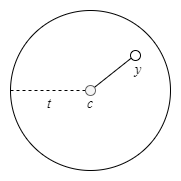
\includegraphics[scale=0.5]{figures/Diagrama_decodificacion_maxima_verosimilitud.png}
    \end{wrapfigure}

    Si la palabra código $c \in \mathcal{C}$ fue enviada y no han ocurrido más de $t$ errores durante la transmisión, el vector recibido es 
    \[
        y = c + e \in \mathbb{F}^n,
    \]
    donde $e$ denota al vector error.
    
    Esto satisface 
    \[
        d(c,y) = d(e,0) \leq t,
    \]
    y por lo tanto $c$ es el único elemento de $\mathcal{C}$ que se encuentra en una bola de radio $t$ alrededor de $y$. Un decodificador de máxima verosimilitud produce este elemento $c$, y así se obtiene el código correcto.
\end{proof}

\begin{definition}
    El \emph{peso de Hamming} $\operatorname{wt}(\mathbf{x})$ de un vector $\mathbf{x} \in \mathbb{F}_q^n$ se define como el número de coordenadas no nulas en $\mathbf{x}$.
\end{definition}

\begin{exampleth}
    Sea $\mathbf{x} = 2001021 \in \mathbb{F}_3^7$ un vector, entonces su peso de Hamming es $wt(\mathbf{x}) = 4$.
\end{exampleth}

El siguiente resultado nos muestra la relación entre la distancia y el peso.

\begin{theorem}
    Si $\mathbf{x}, \mathbf{y} \in \mathbb{F}_q^n$, entonces $\operatorname{d}(\mathbf{x},\mathbf{y}) = \operatorname{wt}(\mathbf{x}-\mathbf{y})$. Si $\mathcal{C}$ es un código lineal, entonces la distancia mínima $d$ coincide con el peso mínimo de las palabras código no nulas de $\mathcal{C}$.
\end{theorem}

\begin{proof}
    Sean $x,y \in \mathbb{F}_q^n$, por la definición de distancia de Hamming tenemos que $d(x,y) = wt(x-y)$. Se supone ahora que $C$ es un código lineal, luego para todo $x,y \in \mathcal{C}$, $x-y \in \mathcal{C}$, luego para cualquier par de elementos $x,y \in \mathcal{C}$, existe $z \in \mathcal{C}$ tal que $d(x,y) = wt(z) \geq wt(\mathcal{C})$, donde $wt(\mathcal{C})$ es el peso mínimo de $\mathcal{C}$. Por tanto, $d \geq wt(\mathcal{C})$. Por otro lado, para todo $x \in \mathcal{C}$, se tiene que $wt(x) = d(x,0)$. Como $\mathcal{C}$ es lineal, $0 \in \mathcal{C}$, luego $d(x,0) \geq d$. Entonces, $wt(\mathcal{C}) \geq d$. Se concluye que $wt(\mathcal{C}) = d$, como se quería.
\end{proof}

Como consecuencia de este teorema, para códigos lineales, la distancia mínima también se denomina \emph{peso mínimo} de un código. Si se conoce el peso mínimo $d$ de un $[n,k]$ código, se dice entonces que es un $[n,k,d]_q$ código.

En el artículo \cite{Vardy_1997} se ha demostrado que el problema de calcular la distancia mínima de un código lineal binario es NP-duro, y el problema de decisión correspondiente es NP-completo.

\begin{problemth}[Distancia mínima]
    \label{pr:min-dist}
    Dada una matriz binaria $H$ de dimensión $m \times n$ y un número entero $w > 0$. ¿Existe un vector no nulo $x \in \mathbb{F}_2^n$ de peso menor que $w$ tal que $Hw^T = 0$? 
\end{problemth}

El problema \ref{pr:min-dist} es un problema NP-completo. Veamos un esquema de la demostración de este resultado. Para ello, haremos uso de una transformación polinomial del problema de Decodificación de Máxima Verosimilitud al problema de Distancia Mínima.

\begin{theorem}[Decodificación de Máxima Verosimilitud]
    \label{th:dmv}
    Dados una matriz binaria $H$ de dimensión $m \times n$, un vector $s \in \mathbb{F}_2^m$ y un número entero $w > 0$. Saber si existe un vector $x \in \mathbb{F}_2^n$ de peso menor o igual que $w$ tal que $Hx^t = s$ es un problema NP-completo.
\end{theorem}

\begin{proof}
    Veamos que este problema es NP-completo reduciendo el problema del emparejamiento tridimensional \cite{Intractability_coding_problems}.

    \begin{problemth}[Emparejamiento Tridimensional]
        Dado un subconjunto $U \subset T \times T \times T$, donde $T$ es un conjunto finito. ¿Existe un conjunto $W \subset U$ tal que $\vert W \vert = \vert T \vert$, y que dos elementos de $W$ no coincidan en alguna coordenada?
    \end{problemth}

    Antes de reducir este problema, vamos a codificar el conjunto $U$ de $3$-tuplas en una matriz de incidencia binaria $\vert U \vert \times 3 \vert T \vert$, en la que cada fila corresponde a una de las $3$-tuplas y tiene peso $3$, y cada $1$ corresponde a una componente de la $3$-tupla. En términos de esta matriz, una solución al problema de Emparejamiento Tridimensional es la existencia de $\vert T \vert$ filas cuya suma módulo $2$ es $111\cdots111$.

    Supongamos entonces que tenemos un algoritmo en tiempo polinómial para el problema de Decodificación de Máxima Verosimilitud. Ahora, dado un conjunto $U \subset T \times T \times T$ para el problema de Emparejamiento Tridimensional, sea $A$ la matriz de incidencia $\vert U \vert \times 3 \vert T \vert$ descrita anteriormente. Entonces, ejecutando el algoritmo para la Decodificación de Máxima Verosimilitud con las entradas $A$, $y = (111\cdots111)$, $w = \vert T \vert$, obtendríamos, en tiempo polinomial, si existen las coincidencias. Esto es, un algoritmo en tiempo polinomial para la Decodificación de Máxima Verosimilitud implica un algoritmo en tiempo polinomial para el Emparejamiento Tridimensional, que a su vez implica un algoritmo en tiempo polinomial para cualquier NP-problema. Esto demuestra que el problema que el problema de Decodificación de Máxima Verosimilitud es NP-completo.
\end{proof}

El problema \ref{th:dmv} es NP-completo y sigue siendo NP-completo bajo ciertas restricciones, luego reformularemos este problema como la versión para cuerpos finitos de Suma de Subconjuntos, un problema NP-completo conocido. Además, calcular la distancia mínima para la clase de códigos lineales sobre un cuerpo de característica 2 es NP-duro, y el problema de decisión correspondiente Distancia Mínima sobre $GF(2^m)$, abreviado $MD_{2^m}$, es NP-completo. Luego esta prueba se basa en una transformación polinomial de Decodificación de Máxima Verosimilitud a $MD_{2^m}$. Sin embargo, esto no prueba que Distancia Mínima sea NP-completo, ya que el posible conjunto de entradas a Distancia Mínima es un pequeño subconjunto del conjunto de posibles entradas a $MD_{2^m}$. Para ello, se construye una aplicación del código $\mathcal{C}$ definido por la matriz de paridad $H$ sobre $GF(2^m)$ a un código binario $\mathbb{C}$, de tal forma que la distancia mínima de $\mathcal{C}$ puede determinarse a partir de la distancia mínima de $\mathbb{C}$. Dado que la longitud de $\mathbb{C}$ está acotada por la longitud de un polinomio de $\mathcal{C}$, y la aplicación en sí se puede lograr en tiempo polinomial, esto completa la prueba de la NP-completitud de Distancia Mínima.

\begin{definition}
    Sea $A_i$, también denotada por $A_i(\mathcal{C})$, el número de palabras código con peso $i$ en $\mathcal{C}$. Se dice que la lista $A_i$ para $0 \leq i \leq n$ es la distribución del peso o espectro del peso de $\mathcal{C}$.
\end{definition}

\section{Clasificación por isometría}

Como hemos visto, las propiedades de un código dependen principalmente de las distancias de Hamming entre sus palabras y entre palabras codificadas y no codificadas. Además, puede ser que un código pueda relacionarse con otro por medio de una aplicación que conserve las distancias de Hamming. De esta forma, podemos definir una relación de equivalencia entre dos códigos que preservan la distancia de Hamming.

Sean $C$ y $C'$ dos $[n,k]_q$ códigos, se dice que son de la \emph{misma cualidad} si existe una aplicación
\[
    \iota : F^n_q \rightarrow F^n_q,
\]
con $\iota(C) = C'$ que preserva la distancia de Hamming, es decir, 
\[
    d(w,w') = d(\iota (w), \iota(w')), \qquad \forall w,w' \in H(n,q).
\]
Las aplicaciones con la propiedad anterior se llaman \emph{isometrías}.

\begin{definition}
    Dos códigos lineales $C, C' \subseteq H(n,q)$ se llaman \emph{isométricos} si existe una isometría de $H(n,q)$ que aplica $C$ sobre $C'$.
\end{definition}

Las permutaciones de las coordenadas son isometrías, que se denominan \emph{isometrías permutacionales}.

\begin{definition}
    Sea $S_n$ el grupo isométrico en el conjunto $X = n = \left\{ 0,..., n-1 \right\}$. Dos códigos lineales $C, C' \subseteq H(n,q)$ son isométricos permutacionalmente si existe una isometría permutacional de $H(n,q)$ que aplica $C$ sobre $C'$. Esto es, hay una permutación $\pi$ en el grupo simétrico $S_n$ tal que 
    \[
        C' = \pi (C) = \left\{ \pi(c) : c \in C \right\}, \quad \text{ and } \quad d(c, \tilde{c}) = d(\pi(c), \pi(\tilde{c})), \qquad \forall c,\tilde{c} \in C,
    \]
    donde
    \[
        \pi(c) = \pi(c_0,...,c_{n-1}) := \left( c_{\pi ^{-1} (0)}, ..., c_{\pi ^{-1} (n-1)} \right).
    \]
\end{definition}

\section{Algoritmo para el cálculo de la distancia}

Como hemos visto, la distancia mínima es importante en un código lineal. Sin embargo, calcular este parámetro para un código dado puede resultar laborioso. A continuación presentaremos el algoritmo de Brouwer-Zimmermann (BZ) para el cálculo de la distancia, que tiene eficiencia exponencial \cite[Sección 1.8]{Wassermann_2006}. Este algoritmo destaca por ser el algoritmo más conocido para calcular la distancia mínima de un código lineal. En particular, si el código es binario se considera eficaz.

\begin{Ualgorithm}[H]
    \DontPrintSemicolon
    \KwIn{$G_1 = (I_k | A_1)$: matriz generadora de $\mathcal{C}$}
    \KwOut{$\bar{d}_i$: distancia mínima}
    $m \longleftarrow 2$\;
    $k_1 \longleftarrow k$\;
    \While{rango$(A_m) \neq 0$}{
        Aplicar la eliminación de Gauss y posibles permutaciones de las columnas de la matriz $A_{m-1}$ desde $G_{m-1} = \left( \begin{array}{c|c} A_{m-1}' & \begin{array}{c|c} I_{k_{m-1}} & A_{m-1} \\ \hline  0 & 0 \end{array} \end{array} \right)$ para obtener la matriz generadora $G_{m} = \left( \begin{array}{c|c}  A_{m}' & \begin{array}{c|c}   I_{k_{m}} & A_{m} \\  \hline 0 & 0  \end{array}  \end{array} \right)$\;
    }
    $C_0 \longleftarrow \left\lbrace 0 \right\rbrace$\;
    $i \longleftarrow 0$\;
    \While{$\bar{d}_i > \underline{d}_i$}{
        $i \longleftarrow i + 1$\;
        $C_i \longleftarrow C_{i-1} \cup \bigcup_{j=1}^m \left\lbrace v \cdot G_j : v \in \mathbb{F}_q^k, \; wt(v) = i \right\rbrace$\;
        $\bar{d}_i \longleftarrow \min \left\{ wt(c) : c \in C_i, \; c \neq 0 \right\}$\;
        $\underline{d}_i \longleftarrow \sum_{\substack{j=1\\ k-k_j \leq i}}^m \left( (i+1)-(k-k_j) \right)$\;
    }
    \caption{Algoritmo de Brouwer-Zimmermann: cálculo de la distancia mínima de un $[n,k]$ código lineal $\mathcal{C}$.}
\end{Ualgorithm}

Veamos, en efecto, que este algoritmo determina la distancia mínima. Consideramos $\mathcal{C}$ un $[n, k]_q$ código lineal y $G$ una matriz generadora. Como el código es lineal, existen matrices $M \in M_n(q)$ y $B \in GL_k(q)$ tales que $B \cdot G \cdot M^T$ es una matriz generadora en forma estándar. De hecho, usando el método de Gauss, podemos obtener una matriz generadora en forma estándar mediante operaciones elementales en las filas y permutaciones de las columnas. En este caso para realizar las operaciones elementales en las filas multiplicaremos desde la izquierda por una matriz $B_1 \in GL_k(q)$, y para permutar las columnas multiplicaremos desde la derecha por la traspuesta de una matriz de permutaciones $M_{\pi_1}$, de tal forma que
$$G_1 := B_1 \cdot G \cdot M_{\pi_1}^T = \left( I_{k_1} | A_1 \right),$$
donde $k_1 = k$.

Ahora que tenemos la matriz generadora en forma estándar, necesitaremos tranformarla de nuevo. Si $A_1$ no es una matriz nula ni vacía, su rango será $k_2$ con $0 < k_2 \leq k_1$. Aplicando la eliminación de Gauss, podemos obtener $k_2$ vectores unitarios diferentes en las $n - k_1$ columnas. Esto es, podemos multiplicar a $G_1$ desde la izquierda por una matriz $B_2 \in GL_k(q)$ y desde la derecha por la traspuesta de una matriz de permutaciones $M_{\pi_2}$ con $\pi_2(j) = j$ para $0 \leq j < k_1$, obteniendo
$$G_2 := B_2 \cdot G_1 \cdot M_{\pi_2}^T = \left( \begin{array}{c|c} A_{2}' & \begin{array}{c|c} I_{k_{2}} & A_{2} \\ \hline  0 & 0 \end{array} \end{array} \right).$$
De esta forma, obtenemos que la matriz $A_2'$ es una matriz $k \times k_1$ y la matriz $A_2$ es una matriz $k_2 \times (n - k_1 - k_2)$. Los ceros indican las matrices nulas.

Una vez que tenemos la matriz generadora de esta forma, realizaremos un procedimiento iterativo aplicando la eliminación de Gauss y posibles permutaciones de las columnas de la matriz $A_2$ hasta que su rango sea 0. Esto es, sea $i \geq 2$, la matriz $A_i$ tiene rango $k_{i+1}$ con $0 < k_{i+1} \leq k_i$. En cada iteración, obtendremos matrices regulares $B_{i+1} \in GL_k(q)$, matrices de permutación $M_{\pi+1} \in M_n(q)$ con $\pi_{i+1}(j) = j$ para $0 \leq j < k_1 + \cdots + k_i$ y matrices generadoras
\[
    G_{i+1} := B_{i+1} \cdot G_i \cdot M_{\pi_{i+1}}^T = \left( \begin{array}{c|c} A_{i+1}' & \begin{array}{c|c} I_{k_{i+1}} & A_{i+1} \\ \hline  0 & 0 \end{array} \end{array} \right),
\]
donde $A_{i+1}'$ es una matriz $k \times (k_1 + \cdots + k_i)$ y $A_{i+1}$ es una matriz $k_{i+1} \times (n - k_1 - \cdots - k_{i+1})$. Repitiendo este procedimiento, finalmente obtendremos una matriz generadora $G_m$ tal que 
\[
    G_{m} = B_m \cdot G_{m-1} \cdot M_{\pi_m}^T = \left( \begin{array}{c|c}  A_{m}' & \begin{array}{c|c}   I_{k_{m}} & A_{m} \\  \hline 0 & 0  \end{array}  \end{array} \right),
\]
donde $A_m$ es una matriz vacía (que significa que no tiene columnas) o es una matriz nula. Entonces, $k_1 + \cdots + k_m \leq n$ y $A_m$ tiene $n - k_1 - \cdots - k_m$ columnas. En consecuencia, la matriz generadora $G_m$ tiene $n - k_1 - \cdots - k_m$ columnas nulas y por lo cual todos los elementos del código generado por $G_m$ tiene peso menor que $k_1 + \cdots + k_m$.

Definimos para $1 \leq i \leq k$ los siguientes conjuntos:
\[
    C_i := \bigcup_{j=1}^m \left\{ v \cdot G_j : v \in \mathbb{F}_q^k, \; wt(v) \leq i \right\}.
\]
Claramente, estos conjuntos forman una cadena ascendente
\[
    C_1 \subseteq \cdots \subseteq C_k,
\]
y por lo tanto los pesos mínimos
\[
    \bar{d}_i := \min \left\{ wt(c) : c \in C_i, \; c \neq 0 \right\}
\]
forman una secuencia decreciente
\[
    \bar{d}_1 \geq \cdots \geq \bar{d}_k = dist(C).
\]
En la mayoría de los casos, no será necesario calcular todos estos valores. En efecto, primero calcularemos $\bar{d}_1$. Después, si $\bar{d}_i$ ya ha sido calculada para algún $i \geq 1$, lo compararemos con $\underline{d}_i$, que es un límite inferior para el peso de los elementos en $C \setminus C_i$. Si $\bar{d}_i \leq \underline{d}_i$, hemos terminado. Si no, repetiremos el mismo proceso para $\bar{d}_{i+1}$.

Para calcular los límites inferiores para los pesos en los complementos $C \setminus C_i$, elegimos un elemento $c \in C \setminus C_i$. Como $c \notin C_i$, entonces existe, para cada $j$, un vector $v^{(j)} \in \mathbb{F}_q^k$ tal que
\[
    c = v^{(j)} \cdot G_j, \quad 1 \leq j \leq m, \; \text{ y } \; wt(v^{(j)}) \geq i + 1.
\]
Para estimar el peso de $c$, nos basaremos en los distintos lugares de información en $G_i$, es decir, las columnas que contienen la matriz identidad $I_{k_j}$. Estas son las columnas de índice $r$ para $k_i + \cdots + k_{j-1} \leq r < k_1 + \cdots + k_j$. Nos interesan las $k_j$ coordenadas $c_r$ de $c = v^{(j)} \cdot G_j$ correspondientes a estas $k_j$ columnas. Como $v^{(j)}$ tiene longitud $k$, estas entradas de $c$ contribuyen al menos el valor de $i + 1 - (k - k_j)$ al peso de $c$. Además, como los conjuntos son disjuntos, para diferentes $j$, tenemos que 
\[
    wt(c) \geq \sum_{j=1}^m \left( i + 1 - (k - k_j) \right).
\]
Restringiendo esta suma a sumandos positivos, obtenemos el límite inferior
\[
    wt(c) \geq \sum_{j \; : \: k - k_j \leq i} \left( i + 1 - (k - k_j) \right) =: \underline{d}_i.
\]
La secuencia de estos límites es incremental, pues el primer sumando es $i + 1$:
\[
    2 \leq \underline{d}_1 < \cdots < \underline{d}_k.
\]
Además,
\[
    \underline{d}_k = m + \sum_{j=1}^m k_j.
\]
Finalmente, como $wt(c) \leq k_1 + \cdots + k_m$ para todo $c \in C$, existe un índice $i_0$ tal que
\[
    \bar{d}_{i_0} \leq \underline{d}_{i_0}.
\]
Para este $i_0$ se cumple que
\[
    \bar{d}_{i_0} := \min \left\{ wt(c) : c \in C_{i_0}, \; c \neq 0 \right\},
\]
y se sigue cumpliendo que 
\[
    \underline{d}_{i_0} \leq \min \left\{ wt(c) : c \in C \setminus C_{i_0} \right\}.
\]
Por lo que
\[
    \bar{d}_{i_0} = dist(C),
\]
y la palabra código de peso $dist(C)$ se encuentra en $C_{i_0}$.

\begin{exampleth}
    Consideramos el $[7, 3]$ código binario $\mathcal{C}$ con matriz generadora 
    \[
        G_1 = \left( 
            \begin{array}{ccc|cccc}
                1 & 0 & 0 & 1 & 0 & 1 & 1 \\ 
                0 & 1 & 0 & 1 & 1 & 0 & 1 \\ 
                0 & 0 & 1 & 0 & 1 & 1 & 1 \\ 
            \end{array}
            \right) .
    \]
    Aplicaremos el algoritmo de BZ para calcular la distancia mínima de este código.

    Observamos que la matriz generadora $G_1$ ya está en forma estándar y su conjunto de información es $\{ 0,1,2 \}$. Luego lo primero que haremos será aplicar el método de Gauss y permutaciones de las columnas para transformar esta matriz generadora en una matriz generadora de la forma
    \[
        \left( \begin{array}{c|c} A_{2}' & \begin{array}{c|c} I_{k_{2}} & A_{2} \\ \hline  0 & 0 \end{array} \end{array} \right),
    \]
    para alguna matriz $A_2'$ de dimensión $3 \times k_1$ y alguna matriz $A_2$ de dimensión $k_2 \times (7 - k_1 - k_2)$. En nuestro caso, tenemos que
    \[
        G_2 := \left( 
            \begin{array}{ccc|ccc|c}
                0 & 1 & 1 & 1 & 0 & 0 & 1 \\ 
                1 & 1 & 0 & 0 & 1 & 0 & 1 \\ 
                1 & 1 & 1 & 0 & 0 & 1 & 0 \\ 
            \end{array}
            \right) .
    \]
    Esta matriz generadora tiene conjunto de información $\{3,4,5\}$. El siguiente paso será realizar de nuevo la eliminación de Gauss y posibles permutaciones de las columnas de la matriz $A_2$ hasta que su rango sea $0$. El algoritmo nos dará la siguiente matriz generadora
    \[
        G_3 := \left( 
            \begin{array}{cccccc|c}
                0 & 1 & 1 & 1 & 0 & 0 & 1 \\ 
                1 & 0 & 1 & 1 & 1 & 0 & 0 \\ 
                1 & 1 & 1 & 0 & 0 & 1 & 0 \\ 
            \end{array}
            \right) .
    \]
    Esta matriz generadora tiene conjunto de información $\{6\}$. El conjunto $C_1$ está formado por las filas de las tres matrices generadoras $G_1$, $G_2$ y $G_3$. Ahora, calculamos el peso de cada uno de ellos, esto es, el número de coordenadas no nulas de cada elemento y obtenemos que todos tienen peso $4$, por lo que $\bar{d}_1 = 4$. El límite inferior del peso mínimo de los vectores que no pertenecen a $C_1$ es $\underline{d}_1 = 1 + 1 - (3-3) + 1 + 1 - (3-3) = 4$. Concluimos que $d = \bar{d}_1 = 4$ es la distancia mínima de $C$.
\end{exampleth}


% 2. Códigos de Goppa.
% Esto lo puedes encontrar en el capítulo 13 de Huffman y Pless. 
% La decodificación  de estos códigos, es similar a la de los códigos BCH (capítulo 5) utilizando el algoritmo de Sugiyama. 
% El artículo donde se definen y se decodifican es el de Goppa.pdf. 
% Además, ahi se explica de forma elemental, sin utilizar geometría algebraica.

\chapter{Códigos de Goppa}

% TODO: introduccion
\textcolor{red}{Hay que completar esta introducción}

Goppa describió una nueva clase de códigos de corrección de errores lineales no cíclicos. Lo más importante es que algunos de estos códigos excedían el límite asintótico de Gilbert-Varshamov, una hazaña que muchos teóricos códigos pensaban que nunca podría lograrse. En este capítulo vamos a hablar sobre los códigos de Goppa y sus propiedades más importantes.


El desarrollo de este capítulo se ha basado en \cite{Huffman_Pless_2010} y \cite{Goppa_codes_1973}.

\section{Algunos códigos clásicos}

Antes de estudiar los códigos de Goppa, introduciremos algunos códigos clásicos para motivar el objetivo de este capítulo.

\subsection{Códigos Reed-Solomon generalizados}

Para $k \geq 0$, $\mathcal{P}_k$ denota el conjunto de polinomios de grado menor que $k$, incluyendo el polinomio nulo, en $\mathbb{F}_q[x]$. Sea $n$ un número entero tal que $1 \leq n \leq q$, $\gamma = (\gamma _0,..., \gamma _{n-1})$ una n-tupla de elementos distintos de $\mathbb{F}_q$, y $\textbf{v} = (v_0,...,v_{n-1})$ una n-tupla de elementos no nulos de $\mathbb{F}_q$. Sea $k$ un número entero tal que $1 \leq k \leq n$. Entonces los códigos

$$GRS_k (\gamma, \textbf{v}) = \left\{ \left( v_0 f(\gamma_0), ..., v_{n-1}f(\gamma_{n-1}) \right) : f \in \mathcal{P}_k \right\}$$

son los códigos Reed-Solomon generalizados (códigos GRS).

\subsection{Códigos clásicos de Goppa}

Los códigos clásicos de Goppa se introdujeron por V. D. Goppa en 1970. Estos códigos son generalizaciones de códigos BCH y subcódigos de subcuerpos de ciertos códigos GRS.

Para motivar la definición de los códigos de Goppa, introduciremos una construcción de los códigos BCH de longitud $n$ sobre $\mathbb{F}_q$. Sea $t = ord_q(n)$ y sea $\beta$ la raíz enésima primitiva de la unidad en $\mathbb{F}_{q^t}$. Elegimos $\delta > 1$ y sea $\mathcal{C}$ el código BCH de longitud $n$ y distancia $\delta$. Entonces $c(x) = c_0 + c_1x + \cdots + c_{n-1}x^{n-1} \in \mathbb{F}_q [x] / (x^n - 1)$ está en $\mathcal{C}$ si y solo si $c(\beta^j) = 0$ para $1 \leq j \leq \delta - 1$. Tenemos que 

$$(x^n - 1) \sum_{i=0}^{n-1} \frac{c_i}{x - \beta ^{-i}} = \sum_{i=0}^{n-1} c_i \sum_{l=0}^{n-1} x^l \left( \beta ^{-i} \right) ^{n-1-l} = \sum_{l=0}^{n-1} x^l \sum_{i=0}^{n-1} c_i \left( \beta^{l+1} \right) ^i.$$

Como $c(\beta^{l+1}) = 0$ para $0 \leq l \leq \delta - 2$, el lado derecho de la ecuación es un polinomio cuyo término de menor grado tiene grado al menos $\delta - 1$. Por lo tanto, el lado derecho se puede escribir como $x^{\delta - 1} p(x)$, donde $p(x)$ es un polinomio en $\mathbb{F}_{q^t}[x]$. Así, podemos decir que $c(x) \in \mathbb{F}_q[x] / (x^n - 1)$ está en $\mathcal{C}$ si y solo si 

$$\sum_{i=0}^{n-1} \frac{c_i}{x - \beta ^{-i}} = \frac{x^{\delta - 1} p(x)}{x^n - 1}$$

o equivalentemente

$$\sum_{i=0}^{n-1} \frac{c_i}{x - \beta ^{-i}} \equiv 0 \pmod{x^{\delta - 1}}$$

La última equivalencia es la base para la definición de los códigos clásicos de Goppa.

Fijado el cuerpo de extensión $\mathbb{F}_{q^t}$ de $\mathbb{F}_q$, sea $L = \{ \gamma_0, ..., \gamma_{n-1} \}$ $n$ elementos distintos de $\mathbb{F}_{q^t}$ y sea $g(x) \in \mathbb{F}_{q^t}[x]$ con $g(\gamma_i) \neq 0$ para $0 \leq i \leq n - 1$. Entonces el \emph{código de Goppa} $\Gamma (L,G)$ es el conjunto de vectores $c_0 \cdots c_{n-1} \in \mathbb{F}_q^n$ tal que 

\begin{equation}
    \label{def:goppa}
    \sum_{i=0}^{n-1} \frac{c_i}{x - \gamma_i} \equiv 0 \pmod{g(x)}
\end{equation}

De esta forma, cuando la parte de la izquierda está escrita como una función racional, significa que el numerador es un múltiplo de $g(x)$. Además, trabajar con módulo $g(x)$ es como trabajar en el anillo $\mathbb{F}_{q^t}[x]/(g(x))$, y la hipótesis $g(\gamma_i) \neq 0$ garantiza que $x - \gamma_i$ es invertible en este anillo. Se llama a $g(x)$ el \emph{polinomio de Goppa} de $\Gamma (L,G)$. Notemos que el código BCH de longitud $n$ y la distancia elegida $\delta$ es el código de Goppa $\Gamma (L,G)$ con $L = \{ 1, \beta^{-1}, ..., \beta^{1-n} \}$ y $g(x) = x^{\delta - 1}$.

A continuación, buscaremos una matriz de paridad para $\Gamma (L,G)$. Para ello, observamos que

$$\frac{1}{x - \gamma_i} \equiv - \frac{1}{g(\gamma_i)} \frac{g(x) - g(\gamma_i)}{x - \gamma_i} \pmod{ g(x)}$$

ya que, comparando numeradores, $1 \equiv - g(\gamma_i)^{-1} \left( g(x) - g(\gamma_i) \right) \pmod{g(x)}$. Así que por \eqref{def:goppa} $\textbf{c} = c_0 \cdots c_{n-1} \in \Gamma (L,G)$ si y solo si

\begin{equation}
    \label{congruencia_goppa}
    \sum_{i=0}^{n-1} c_i \frac{g(x) - g(\gamma_i)}{x - \gamma_i} g(\gamma_i)^{-1} \equiv 0 \pmod{g(x)}
\end{equation}

Supongamos que $g(x) = \sum_{j=0}^w g_j x^j$ con $g_j \in \mathbb{F}_{q^t}$, donde $w = gr(g(x))$. Entonces

$$\frac{g(x) - g(\gamma_i)}{x - \gamma_i} g(\gamma_i)^{-1} = g(\gamma_i)^{-1} \sum_{j=1}^w g_j \sum_{k=0}^{j-1} x^k \gamma_i^{j-1-k} = g(\gamma_i)^{-1} \sum_{k=0}^{w-1} x^k \left( \sum_{j=k+1}^w g_j \gamma_i^{j-1-k} \right)$$

Por lo tanto, por \eqref{congruencia_goppa}, estableciendo los coeficientes de $x^k$ iguales a $0$, en el orden $k = w - 1, w - 2, ..., 0$, tenemos que $\textbf{c} \in \Gamma (L,G)$ si y solo si $Hc^T = 0$, donde 

\begin{equation}
    H = \left(
        \begin{array}{ccc} 
            h_0 g_w & \cdots & h_{n-1} g_w  \\
            h_0 (g_{w-1} + g_w \gamma_0) & \cdots & h_{n-1} (g_{w-1} + g_w \gamma_{n-1}) \\
            & \vdots & \\
            h_0 \sum_{j=1}^w \left( g_j + \gamma_0^{j-1} \right) & \cdots & h_{n-1} \sum_{j=1}^w \left( g_{j} + \gamma_{n-1}^{j-1} \right) \\
        \end{array}
        \right)
\end{equation}

con $h_i = g(\gamma_i)^{-1}$.

\begin{proposition}
    La matriz $H$ se puede reducir a una matriz $H'$ de dimensión $w \times n$, donde 

    \begin{equation}
        H' = \left(
            \begin{array}{ccc} 
                g(\gamma_0)^{-1} & \cdots & g(\gamma_{n-1})^{-1}  \\
                g(\gamma_0)^{-1} \gamma_0 & \cdots & g(\gamma_{n-1})^{-1} \gamma_{n-1} \\
                & \vdots & \\
                g(\gamma_0)^{-1} \gamma_0^{w-1} & \cdots & g(\gamma_{n-1})^{-1} \gamma_{n-1}^{w-1} \\
            \end{array}
            \right)
    \end{equation}
\end{proposition}

Las entradas de $H'$ están en $\mathbb{F}_{q^t}$. Eligiendo una base de $\mathbb{F}_{q^t}$ sobre $\mathbb{F}_q$, cada elemento de $\mathbb{F}_{q^t}$ se puede representar como un vector columna $t \times 1$ sobre $\mathbb{F}_q$. Reemplazando cada entrada de $H'$ por su correspondiente vector columna, obtenemos una matriz $H''$ de dimensión $tw \times n$ sobre $\mathbb{F}_{q}$ que tiene la propiedad de que si $\textbf{c} \in \mathbb{F}_q^n$ está en $\Gamma(L, G)$ si y solo si $H''c^T = 0$.

El siguiente resultado nos muestra los límites en la dimensión y la distancia mínima de un código de Goppa.

\begin{theorem}
    Con la notación de esta sección, sea $\Gamma (L, G)$ un código de Goppa tal que $gr(g(x)) = w$ entonces es un $[n, k, d]$ código con $k \geq n - wt$ y $d \geq w + 1$.
\end{theorem}

\begin{proof}
    Las filas de $H''$ pueden ser dependientes, luego esta matriz tiene rango como máximo $wt$. Por lo que $\Gamma(L,G)$ tiene dimensión al menos $n - wt$. Si una palabra código $\textbf{c} \in \Gamma (L, G)$ tiene peso $w$ o menos, entonces el lado izquierdo de \ref{def:goppa} es una función racional, donde el numerador tiene grado $w - 1$ o menos; pero este numerador tiene que ser múltiplo de $g(x)$, lo cual es una contradición pues el grado de $g$ es $w$.
\end{proof}

Sin embargo, si nos restringimos sobre ciertos polinomios y el cuerpo $\mathbb{F}_2$, podemos garantizar una distancia mínima de $2w + 1$.



\section{Decodificación de los códigos de Goppa}

Como hemos visto, al transmitir una palabra código a un receptor, éste podría recibir la palabra alterada. Para que el receptor pueda determinar el mensaje original, necesitaremos decodificar el mensaje recibido. Supongamos que $E$ es el vector de errores que se añade a la palabra código $C$ transmitida, entonces la palabra recibida $R$ está dada por

$$R = C + E$$

de donde 

$$\sum_{\gamma \in L} \frac{R_\gamma}{x - \gamma} = \sum_{\gamma \in L} \frac{C_\gamma}{x - \gamma} + \sum_{\gamma \in L} \frac{E_\gamma}{x - \gamma}.$$

Como $C$ es una palabra código, la primera sumatoria de la parte derecha desaparece al aplicar el módulo $g(x)$, y tenemos que

$$\sum_{\gamma \in L} \frac{R_\gamma}{x - \gamma} = \sum_{\gamma \in L} \frac{E_\gamma}{x - \gamma} \pmod{g(x)}.$$

Definiremos su síndrome como el polinomio $S(x)$ de grado menos que $gr(g(x))$ tal que 

$$S(x) = \sum_{\gamma \in L} \frac{R_\gamma}{x - \gamma} \pmod{g(x)}.$$

Acabamos de ver que 

$$S(x) = \sum_{\gamma \in L} \frac{E_\gamma}{x - \gamma} \pmod{g(x)}.$$

Sea $M$ un subconjunto de $L$ tal que $E_{\gamma} \neq 0$ si y solo si $\gamma \in M$. Entonces

\begin{equation}
    \label{def:sindrome}
    S(x) = \sum_{\gamma \in M} \frac{E_\gamma}{x - \gamma} \pmod{g(x)}.
\end{equation}

De esta forma, ahora podemos introducir el polinomio cuyas raíces son las ubicaciones de los errores,

\begin{equation}
    \label{def:localizaciones}
    \sigma (x) = \prod_{\gamma \in M} (x - \gamma)
\end{equation}

Sin embargo, para los códigos de Goppa es más conveniente definir una variante de este polinomio de la siguiente forma.

\begin{equation}
    \label{def:eta}
    \eta (x) = \sum_{\gamma \in M} E_\gamma \prod_{\partial \in M \setminus \{ \gamma \} } (x - \partial)
\end{equation}

Observemos que de esta forma $\sigma(x)$ y $\eta(x)$ deben ser primos relativos.

Derivando la expresión de $\sigma(x)$, tenemos que 

\begin{equation}
    \label{def:localizaciones_derivada}
    \sigma'(x) = \sum_{\gamma \in M} \prod_{\partial \in M \setminus \{ \gamma \} } (x - \partial)
\end{equation}


de donde, para cada $\gamma \in M$,

$$\eta (\gamma) = E_\gamma \prod_{\partial \in M \setminus \{ \gamma \} } (\gamma - \partial) = E_\gamma \sigma'(\gamma)$$

por lo que $E_\gamma = \frac{\eta(\gamma)}{\sigma'(\gamma)}$. De esta forma, una vez que hemos calculado los polinomios $\sigma$ y $\eta$, las coordenadas del vector error vienen dadas por 

\[
    E_\gamma = \left\{ \begin{array}{lcc}
    0 &   \text{si}  & \sigma(\gamma) \neq 0 \\
    \\ \frac{\eta(\gamma)}{\sigma'(\gamma)} &  \text{si} & \sigma(\gamma) = 0
    \end{array}
    \right.
\]

donde $\sigma'(x)$ es la derivada de $\sigma(x)$.

Lo esencial para decodificar los códigos de Goppa es determinar los coeficientes de los polinomios $\sigma$ y $\eta$. Para ello, tenemos que relacionar $\sigma$ y $\eta$ al síndrome de la ecuación \ref{def:sindrome}. Esto se consigue multiplicando las ecuaciones \ref{def:sindrome} y \ref{def:localizaciones}, obteniendo

\begin{equation}
    \label{prop:key_equation}
    S(x) \cdot \sigma(x) \equiv \eta(x) \pmod{g(x)}
\end{equation}

La ecuación \ref{prop:key_equation} es la \emph{ecuación clave} para decodificar los códigos de Goppa. Dado $g(x)$ y $S(x)$, el problema de decodificar consiste en encontrar polinomios de grado bajo $\sigma(x)$ y $\eta(x)$ que satisfacen \ref{prop:key_equation}.

Reduciendo cada potencia de $x \pmod{g(x)}$ e igualando coeficientes de $1, x, ..., x^{gr g - 1}$, tenemos que \ref{prop:key_equation} es un sistema de $gr G$ ecuaciones lineales donde las incógnitas son los coeficientes de $\sigma$ y $\eta$. Por lo tanto, para probar que el decodificador es capaz de corregir todos los patrones hasta $t$ errores, basta con probar que \ref{prop:key_equation} tiene una única solución con grados de $\sigma$ y de $\eta$ suficientemente pequeños. Esto equivale a que el conjunto de ecuaciones lineales correspondientes sean linealmente independientes.

Supongamos que existen dos pares diferentes de soluciones a \ref{prop:key_equation}:

\begin{equation}
    \label{prop:key_equation_1}
    S(x) \sigma^{(1)}(x) \equiv \eta^{(1)}(x) \pmod{g(x)}
\end{equation}

\begin{equation}
    \label{prop:key_equation_2}
    S(x) \sigma^{(2)}(x) \equiv \eta^{(2)}(x) \pmod{g(x)}
\end{equation}

donde $\sigma^{(1)}(x)$ y $\eta^{(1)}(x)$ son primos relativos, al igual que $\sigma^{(2)}(x)$ y $\eta^{(2)}(x)$. Además, $\sigma^{(1)}(x)$ y $g(x)$ no pueden tener ningún factor en común, pues en ese caso ese factor podría dividir a $\eta^{(1)}(x)$, contradiciendo que $\sigma^{(1)}(x)$ y $\eta^{(1)}(x)$ son primos relativos. Así, podemos dividir \ref{prop:key_equation_1} por $\sigma^{(1)}(x)$ y obtenemos

$$S(x) \equiv \frac{\eta^{(1)}(x)}{\sigma^{(1)}(x)} \pmod{g(x)}$$

de la misma forma para \ref{prop:key_equation_2},

$$S(x) \equiv \frac{\eta^{(2)}(x)}{\sigma^{(2)}(x)} \pmod{g(x)}$$

de donde,

\begin{equation}
    \label{prop:key_equation_12}
    \sigma^{(1)}(x) \eta^{(2)}(x) \equiv \sigma^{(2)}(x) \eta^{(1)}(x) \pmod{g(x)}
\end{equation}

Si $gr(G) = 2t$ y $gr(\sigma^{(1)}) \leq t$, $gr(\sigma^{(2)}) \leq t$, $gr(\eta^{(2)}) < t$ y $gr(\eta^{(1)}) < t$, entonces se da la siguiente igualdad

\begin{equation}
    \label{prop:key_equation_caso1}
    \sigma^{(1)}(x) \eta^{(2)}(x) = \sigma^{(2)}(x) \eta^{(1)}(x)
\end{equation}

Así, $\sigma^{(1)}$ divide a $\sigma^{(2)} \eta^{(1)}$, y como $\sigma^{(1)}$ y $\eta^{(1)}$ son primos relativos, $\sigma^{(1)}$ tiene que dividir a $\sigma^{(2)}$. Análogamente, $\sigma^{(2)}$ tiene que dividir a $\sigma^{(1)}$. Como ambos son mónicos, se tiene que $\sigma^{(1)} = \sigma^{(2)}$ y así, $\eta^{(1)} = \eta^{(2)}$. Con esto hemos probado que si el grado de $G$ es $2t$, entonces \ref{prop:key_equation} tiene una única solución cuando $gr(\eta) < gr(\sigma) \leq t$, luego el correspondiente sistema de ecuaciones lineales donde las incógnitas son los coeficientes de $\sigma$ y $\eta$ tiene que ser no singular. En el siguiente teorema se concluye este resultado.

\begin{theorem}
    Si $gr(g(x)) = 2t$, entonces hay un algoritmo de decodificación algebraica de corrección de $t$ errores para el código q-ario de Goppa con el polinomio de Goppa $g(x)$.
\end{theorem}

Estudiemos ahora este resultado en el caso binario, primero observamos que ya que todos los $E_\gamma$ distintos de cero son iguales a 1, entonces \ref{def:eta} y \ref{def:localizaciones_derivada} coincidan. De esta forma, la ecuación \ref{prop:key_equation_12} ahora pasa a ser

$$\sigma^{(1)} \left( \sigma^{(2)} \right) ' \equiv \sigma^{(2)} \left( \sigma^{(1)} \right) ' \pmod{g(x)}$$

Ahora, cuando $\sigma$ sea par escribiremos en su lugar $\hat{\sigma}$, mientras que cuando $\sigma$ sea impar escribiremos en su lugar $x \sigma '$. Así, tenemos que

\begin{align*} 
    \left( \hat{\sigma}^{(1)} + x \sigma^{(1)'} \right) \sigma^{(2)'} &\equiv \left( \hat{\sigma}^{(2)} + x \sigma^{(2)'} \right) \sigma^{(1)'}\\ 
    \hat{\sigma}^{(1)} \sigma^{(2)'} + \hat{\sigma}^{(2)} \sigma^{(1)'} &\equiv 0 \pmod{g(x)}.
\end{align*}

El lado izquierdo es un cuadrado perfecto, pues todos los polinomios de ese lado son pares. Esto implica que

$$\hat{\sigma}^{(1)} \sigma^{(2)'} + \hat{\sigma}^{(2)} \sigma^{(1)'} \equiv 0 \pmod{\bar{G}(x)}$$

donde $\bar{G}(x)$ es múltiplo de $g(x)$ de menor grado ya que $\bar{G}$ es un cuadrado perfecto. Por lo que, si $gr(\bar{G}) = 2t$, $gr(\sigma^{(1)}) \leq t$ y $gr(\sigma^{(2)}) \leq t$, entonces 

$$\hat{\sigma}^{(1)} \left( \sigma^{(2)} \right) ' = \hat{\sigma}^{(2)} \sigma^{(1)'}.$$

Por la primalidad relativa, $\sigma^{(1)} = \sigma^{(2)}$. En el siguiente teorema se concluye este resultado.

\begin{theorem}
    Si $gr(g(x)) = t$ y si $g(x)$ no tiene factores irreducibles repetidos, entonces hay un algoritmo de decodificación algebraica de corrección de $t$ errores para el código de Goppa binario con el polinomio de Goppa $g(x)$.
\end{theorem}


%% 4. Criptografía post-cuántica basada en códigos. 
% Aquí depende de si vas a matricularte en la asignatura de Criptografía (la imparte Javier Lobillo). 
% Allí te explicarán los sistemas asimétricos. Si no te matriculas, lo puedes encontrar en el libro Introduction to Cryptography (capítulos 1,2,3).
% No te hace falta todo lo que hay en esos capítulos, pero, bueno, es interesante para una matemática/informática el conocer este tipo de cosas.
% Para la parte post-cuántica, tenemos el archivo 9783540887010-c1.pdf y el libro Post-QuantumCryptography 
% (capítulos Introduction to post-quantum cryptography y Code-based cryptography, también Quantum computing, si te apetece). 
% Para el criptosistema de McEliece (que es que implementaremos) está el archivo sander-report-s15.pdf, 
% donde se explica este y el criptosistema de Niederreiter, que es equivalente en seguridad.

% buscar la referencia original del 78 de McEliece que ahi viene mejor explicado

\chapter{Criptografía post-cuántica basada en códigos}

El principal objetivo de la criptografía es proporcionar confidencialidad mediante métodos de cifrado. Cuando queremos enviar un mensaje a un destinatario, el canal de comunicación puede ser inseguro y otras personas podrían leerlo o incluso modificarlo de tal forma que el destinatario no se diera cuenta. Para prevenir estos ataques nos será de utilidad la criptografía.

En este capítulo introduciremos las nociones básicas de la criptografía, junto a sus objetivos, y estudiaremos los dos principales tipos de criptosistemas (simétricos y asimétricos) \cite{Introduction_to_cryptography}. Definiremos el primer y más utilizado algoritmo de los sistemas criptográficos asimétricos, el RSA. Finalmente, discutiremos la seguridad de los criptosistemas ante la existencia de ordenadores cuánticos y mostraremos algunas alternativas que sean capaces de resistir sus ataques \cite{Post-Quantum_Cryptography_2009}. En concreto, estudiaremos el criptosistema de McEliece y el de Niederreiter \cite{Sander}.

\section{Introducción}

En general, los métodos de cifrado consisten en encriptar un mensaje, llamado \emph{texto plano}, antes de ser transmitido, de esta forma obtenemos un \emph{texto cifrado} o \emph{criptograma}. Este texto cifrado se transmite al destinatario, quien lo \emph{desencripta} mediante una \emph{clave de descifrado}, la cual solo conocen el receptor y el emisor, que previamente ha sido intercambiada.

Formalmente, dado un conjunto de los mensajes $\mathcal{M}$, un conjunto de los criptogramas $\mathcal{C}$ y el espacio de claves $\mathcal{K}_p \times \mathcal{K}_s$, un \emph{criptosistema} viene definido por dos aplicaciones
\[
    E : \mathcal{K}_p \times \mathcal{M} \rightarrow \mathcal{C},
\]
\[
    D : \mathcal{K}_s \times \mathcal{C} \rightarrow \mathcal{M},
\]
tales que para cualquier clave $k_p \in \mathcal{K}_p$, existe una clave $k_s \in \mathcal{K}_s$ de manera que dado cualquier mensaje $m \in \mathcal{M}$,
\begin{equation}
    \label{def:criptosistema}
    D(k_s, E(k_p, m)) = m.
\end{equation}

Para simplificar la notación de las funciones de cifrado y descifrado usaremos, fijadas las claves $k_p \in \mathcal{K}_p$ y su correspondiente $k_s \in \mathcal{K}_s$:
\begin{align*} 
    E_{k_p} &: \mathcal{M} \rightarrow \mathcal{C}, \quad [ E_{k_p} (m) = E(k_p, m) ]\\ 
    D_{k_s} &: \mathcal{C} \rightarrow \mathcal{M}, \quad [ D_{k_s} (c) = D(k_s, c) ]
\end{align*}

La propiedad \ref{def:criptosistema} se transforma en
\[
    D_{k_s} \left( E_{k_p}(m) \right) = m.
\]
Para encriptar y desencriptar existen \emph{algoritmos de cifrado} y \emph{de descifrado}, respectivamente, y cada uno usará una clave secreta. Si esta clave es la misma en ambos algoritmos, diremos que los métodos de encriptación son \emph{simétricos}. Algunos ejemplos importantes de estos métodos son DES (\emph{Data Encryption Standard}) y AES (\emph{Advanced Encryption Standard}).

En 1976, Diffie y Hellman \cite{Diffie_Hellman_1976} introdujeron un concepto revolucionario, la \emph{criptografía de Clave Pública}, también llamada \emph{criptografía asimétrica}, que permitió dar una solución al antiguo problema del intercambio de claves e indicar el camino a la firma digital. Los métodos de cifrado de \emph{clave pública} son \emph{asimétricos}. Cada receptor tiene una clave personal $k = (k_p, k_s)$, que consiste en dos partes: $k_p$ es la clave de cifrado y es pública, y $k_s$ es la clave de descifrado, que es privada. De esta forma, si queremos enviar un mensaje, lo encriptaremos mediante la clave pública $k_p$ del receptor. Así, el receptor poddrá descifrar el texto cifrado usando su clave privada $k_s$, que solo conoce él. Al ser la clave pública, cualquiera puede encriptar un mensaje usándola, sin embargo descifrarlo sin saber la clave privada será casi imposible.

\section{Objetivos de la criptografía}

Además de proporcionar confidencialidad, la criptografía proporciona soluciones para otros problemas:

\begin{enumerate}
    \item \emph{Confidencialidad}. La información solo puede ser accesible por las entidades autorizadas.
    \item \emph{Integridad de datos}. El receptor de un mensaje debería ser capaz de determinar que el mensaje no ha sido modificado durante la transmisión.
    \item \emph{Autenticidad}. El receptor de un mensaje debería ser capaz de verificar su origen.
    \item \emph{No repudio}. El emisor de un mensaje debería ser incapaz de negar posteriormente que envió el mensaje.
\end{enumerate}

Para garantizar la integridad de los datos, hay métodos simétricos y de clave pública. El mensaje $m$ es aumentado por un \emph{código de autenticación de mensaje} (MAC). Este código es generado por un algoritmo que depende de la clave secreta. Así, el mensaje aumentado $(m, MAC(k,m))$ está protegido contra modificaciones. El receptor ahora puede comprobar la integridad del mensaje $(m, \bar{m})$ verificando que $MAC(k, m) = \bar{m}$.

Las firmas digitales requieren métodos de clave pública y proporcionan autenticación y no repudiablidad. Cualquier persona puede verificar si una firma digital es válida con la clave pública del firmante. Esto es, si firmamos con nuestra clave privada $k$, obtenemos la firma $Sign(k_s, m)$. El receptor recibe la firma $s$ del mensaje $m$ y comprueba con el algoritmo de verificación \emph{Verify} que se cumple que \emph{Verify}$(k_p, s, m) = ok$, siendo $k_p$ la clave pública del emisor.

\section{Criptografía simétrica}

Un criptosistema \emph{simétrico}, como hemos visto, viene determinado por dos aplicaciones
\[
    E : \mathcal{K} \times \mathcal{M} \rightarrow \mathcal{C},
\]
\[
    D : \mathcal{K} \times \mathcal{C} \rightarrow \mathcal{M},
\]
tales que para cualquier clave $k \in \mathcal{K}$ y cualquier mensaje $m \in \mathcal{M}$,
\begin{equation}
    \label{def:criptosistema_simetrico}
    D(k, E(k, m)) = m.
\end{equation}

Fijada $k \in \mathcal{K}$, usaremos la notación 
\[
    E_k : \mathcal{M} \rightarrow \mathcal{C},
\]  
\[
    D_k : \mathcal{C} \rightarrow \mathcal{M},
\]
para las funciones de cifrado y descifrado. La propiedad \ref{def:criptosistema_simetrico} se transforma en
\[
    D_k \left( E_k (m) \right) = m.
\]
Observamos que la clave que se usa para cifrar es la misma que se usa para descifrar.

Algunos ejemplos importantes de sistemas simétricos son DES (\emph{Data Encryption Standard}) y AES (\emph{Advanced Encryption Standard}) \cite[Sección 2.1]{Introduction_to_cryptography}.

\section{Criptografía asimétrica}

A diferencia de la criptografía simétrica, en la criptografía asimétrica los participantes en la comunicación no comparten una clave secreta. Cada uno tiene un par de claves: la \emph{clave secreta} $k_s$ conocida solo por él y una \emph{clave pública} conocida por todos.

Supongamos que Bob tiene un par de claves $(k_p, k_s)$ y Alice quiere encriptar un mensaje $m$ para Bob. Alice, como cualquier otra persona, conoce la clave pública $k_p$ de Bob. Alice usa una función de encriptación $E$ con la clave pública $k_p$ de Bob para obtener el texto cifrado $c = E_{k_p}(m)$. Esto solo puede ser seguro si es prácticamente inviable calcular $m$ de $c = E_{k_p}(m)$. Sin embargo, Bob sí es capaz de calcular el mensaje $m$, ya que puede usar su clave secreta. La función de encriptación $E_{k_p}$ debe tener la propiedad de que su pre-imagen $m$ del texto cifrado $c = E_{k_p}(m)$ sea fácil de calcular usando la clave secreta $k_s$ de Bob, quien es el único que puede descifrar el mensaje encriptado.

En la criptografía de clave pública, necesitamos unas funciones $\left( E_{k_p} \right)_{k_p \in K_P}$ tales que cada función $E_{k_p}$ se pueda cacular con un algoritmo eficiente. Sin embargo, su pre-imagen debería ser prácticamente inviable de calcular. Estas familias $\left( E_{k_p} \right)_{k_p \in K_P}$ se denominan \emph{funciones de una sola dirección}. En cada función $E_{k_p}$ de la familia, tiene que haber una información secreta $k_s$ para que el algoritmo sea eficiente y calcule la inversa de $E_{k_p}$. Las funciones con esa propiedad se denominan \emph{funciones con trampilla}.

En 1976, Diffie y Hellman \cite{Diffie_Hellman_1976} presentaron la idea de la criptografía de clave pública, es decir, introdujeron métodos de clave pública para el acuerdo de clave y, además, describieron cómo las firmas digitales funcionarían. El primer criptosistema de clave pública que podía servir como un mecanismo de acuerdo de clave y como una firma digital fue el criptosistema RSA, que actualmente es el más conocido y usado. Este criptosistema lleva el nombre de sus inventores: Rivest, Shamir y Adleman. El criptosistema RSA se basa en la dificultad de factorizar grandes números, lo que le permite construir funciones de una sola dirección con una trampilla. Otras funciones de una sola dirección se basan en la dificultad de extraer logaritmos discretos. Estos dos problemas de la teoría de números son los cimientos de los criptosistemas de clave pública más usados actualmente.

Cada participante en un criptosistema de clave pública tiene una clave $k = (k_p, k_s)$, que consiste en una clave pública ($k_p$) y una clave privada o secreta ($k_s$). Para garantizar la seguridad del criptosistema, debería ser inviable obtener la clave privada $k_s$ a partir de la clave pública $k_p$. Un algoritmo eficiente debería ser el encargado de elegir aleatoriamente ambas claves en un gran espacio de parámetros. Así, cualquiera puede usar $k_p$ para encriptar mensajes, pero solo quien posea $k_s$ podrá desencriptarlos.

En cuanto a las firmas digitales, supongamos que tenemos una familia de funciones con trampilla $\left( E_{k_p} \right)_{k_p \in K_P}$ donde cada función $E_{k_p}$ es biyectiva. Sea $k_p$ la clave pública de Alice, quien es la única capaz de calcular la inversa $E_{k_p}^{-1}$ de $E_{k_p}$ pues para ello se necesita la clave privada $k_s$ de Alice. De esta forma, si Alice quiere firmar un mensaje $m$, tiene que calcular $E_{k_p}^{-1}(m)$, que será el valor de la firma $s$ de $m$. Todo el mundo puede verificar la firma de Alice $s$ pues cualquiera puede usar su clave pública $k_p$ y calcular $E_{k_p}(s)$. Si $E_{k_p} (s) = m$, entonces podemos asegurarnos de que Alice realmente firmó $m$ porque es la única que es capaz de calcular $E_{k_p}^{-1}(m)$.

Una importante aplicación de los criptosistemas de clave pública es que permiten intercambiar claves en sistemas de clave secreta. Si Alice conoce la clave pública de Bob, ella puede generar una clave de sesión, cifrarla con la clave pública de Bob y enviársela.  

Algunos sistemas conocidos de clave pública son:

\begin{itemize}
    \item \emph{RSA}: está basado en el problema de factorización de enteros.
    \item \emph{ElGamal}: está basado en el problema del logaritmo discreto.
    \item \emph{McEliece}: está basado en la teoría de los códigos Goppa.
    \item \emph{Curvas Elípticas}: son una generalización del sistema ElGamal y se basan en el problema de calcular logaritmos discretos en curvas elípticas.
\end{itemize}

\subsection{RSA}

El criptosistema RSA consiste en multiplicar dos números primos muy grandes y publicar su producto $n$. Una parte de la clave pública la conformará $n$, mientras que los factores de $n$ se mantienen en secreto y se usarán como clave privada. La idea básica es que los factores de $n$ no puedan recuperarse de $n$ en un tiempo razonable. Por lo que la seguridad de RSA radica en la dificultad del problema de factorización de enteros.

\subsubsection{Generación de claves}

Cada usuario del criptosistema RSA posee una clave pública y otra privada. Para generar este par de claves, se siguen los siguientes tres pasos:

\begin{enumerate}
    \item Se eligen aleatoriamente dos grandes números primos distintos $p$ y $q$ y se calcula su producto $n = p \cdot q$. También calculamos $\phi(n) = n + 1 - (p + q)$.
    \item Se elige un entero $e$ tal que $1 < e < \phi(n)$ y sea primo con $\phi(n)$.
    \item Se calcula $d$ que verifique $ed \equiv 1 \pmod{\phi(n)}$, es decir, $d \equiv e^{-1} \pmod{\phi(n)}$. 
    \item La clave privada es $(p, q, d)$.
    \item La clave pública es $(n, e)$.
\end{enumerate}

Los números $n$, $e$ y $d$ se denominan \emph{módulo}, \emph{exponente de cifrado} y \emph{exponente de descifrado}, respectivamente. El exponente de descifrado $d$ se puede obtener con el algoritmo extendido de Euclides. Con este exponente es posible descifrar un texto cifrado y generar una firma digital.

\subsubsection{Cifrado y descifrado}

Supongamos que queremos cifrar un mensaje. Para ello, usaremos la clave pública $(n, e)$. Para cifrar un texto plano $m$ podemos usar la función de cifrado:
\[
    RSA_{n, e}(m) = m^e \pmod{n},
\]
es decir, el texto cifrado $c$ es $m^e$ módulo $n$.

Para descifrar el criptograma $c$, se usa la función de descifrado:
\[
    RSA_{n, d}(c) = c^d \pmod{n}.
\]
De esta forma, se puede recuperar el texto plano, es decir, $m = c^d$ módulo $n$, pues las funciones de cifrado y descifrado $RSA_{n, e}$ y $RSA_{n, d}$ son inversas entre sí.

Con este procedimiento de cifrado, podemos cifrar secuencias de bit hasta $k := \lfloor \log_2{n} \rfloor$ bits. Si los mensajes son más largos, podemos dividirlos en bloques de longitud $k$ y cifrar cada uno por separado.

\begin{exampleth}
    Consideremos dos números primos $p = 7$ y $q = 11$, tenemos que $n = p \cdot q = 77$ y $\phi(n) = 60$. Busquemos ahora un número $e$ mayor que $1$ y menor que $60$ y que sea primo con $\phi(n) = 60$, elegimos $e = 13$. Por lo que el exponente de descifrado es
    \[
        d \equiv e^{-1} \equiv 37 \mod{\phi(n)}.
    \]
    La clave pública es $(e, n) = (13, 77)$ y la clave privada es $(d, n) = (37, 77)$. Vamos a cifrar el mensaje $m = 42$ con la función de cifrado:
    \[
        RSA_{n, e}(m) = m^e \equiv 42^{13} \equiv 14 \pmod{n}.
    \]
    Luego el mensaje cifrado $m$ es $14$. Ahora, si queremos descifrarlo, calcularemos lo siguiente:
    \[
        RSA_{n, d}(c) = c^d \equiv 14^{37} \equiv 42 \pmod{n}.
    \]
    Observamos que efectivamente coincide con el mensaje original $m$.
\end{exampleth}

\subsubsection{Firma digital}

El criptosistema RSA también se puede usar para realizar firmas digitales. Sea $(n, e)$ la clave pública y $d$ el exponente de descifrado, si queremos firmar un mensaje $m$, le aplicamos el algoritmo de descifrado y obtenemos la \emph{firma} de $m$, $\sigma = m^d$. Decimos que $(m, \sigma)$ es un \emph{mensaje firmado}. Para verificar ese mensaje, basta con calcular $\sigma ^e$, donde $e$ es la clave pública del firmante, y comprobar que coincide con $m$.

\section{Criptografía post-cuántica}

En \cite{Post-Quantum_Cryptography_2009} se comenta la creencia de que algunos sistemas criptográficos, tales como RSA, resisten los ataques de ordenadores clásicos, pero no de los ordenadores cuánticos. Sin embargo, se cree que algunas alternativas, como el sistema de McEliece con una clave de cuatro millones de bits, son capaces de resistir los ataques de ordenadores clásicos y cuánticos. Es por esto que surgen diversas preocupaciones ante la amenaza de los ordenadores cuánticos: se duda sobre si seguir usando RSA o simplemente cambiar a otros sistemas criptográficos que sean resistentes a dichos ordenadores. Sin embargo, esto último no es tan sencillo pues necesitamos tiempo para mejorar la eficiencia, fomentar la confanza y mejorar de la usabilidad de los criptosistemas post-cuánticos. En resumen, todavía no estamos preparados para que el mundo cambie a la criptografía post-cuántica.

En esta sección estudiaremos los sistemas criptográficos basados en códigos, es decir, criptosistemas que usan una familia de códigos correctores de errores $\mathcal{C}$. Para ello, agregan un error a una palabra de alguno de los códigos $\mathcal{C}$ o al calcular un síndrome relativo a la matriz de paridad de $\mathcal{C}$.

El primer criptosistema desarrollado es un sistema de cifrado de clave pública y fue propuesto por Robert J. McEliece en 1978 \cite{McEliece_1978}. Este sistema esencialmente usa como clave privada un código de Goppa binario aleatorio y, como clave pública, una matriz generadora de una versión permutada aleatoriamente de ese código. El texto cifrado es una palabra código a la que se le han añadido algunos errores, y solo el que posee la clave privada puede eliminar esos errores en un tiempo razonable. Actualmente, no se conoce ningún ataque que presente una amenaza grave a este sistema, ni siquiera utilizando un ordenador cuántico. Cabe destacar la seguridad y la rapidez del criptosistema de McEliece, ya que tanto los procedimientos de cifrado y descifrado son de baja complejidad.

\subsection{Criptosistema de McEliece}

En 1978, R. J. McEliece propuso un criptosistema de clave pública \cite{McEliece_1978}. El criptosistema de McEliece se basa en códigos lineales de corrección de errores y hasta ahora es el criptosistema más exitoso basado en nociones de teoría de codificación.

La construcción original en \cite{McEliece_1978} usa códigos de Goppa binarios para cifrar y descifrar mensajes. Sim embargo, han surgido otras variantes de este criptosistema que usan otros códigos lineales, pero la mayoría han resultado ser inseguros. A día de hoy, la construcción original de 1978 se considera segura con la correcta elección de parámetros.

Por esta razón, el criptosistemade McEliece se pone a la altura del RSA. Existen algunas diferencias entre ambos criptosistemas, el de McEliece es capaz de cifrar y descifrar mensajes más rápido. Sin embargo, los tamaños de las claves son mayores que los del RSA, que es la razón por la que el criptosistema de McEliece apenas se usa. La principal razón por la que está creciendo el interés en el criptosistema de McEliece es porque es uno de los mejores candidatos para criptosistemas de clave pública seguros post-cuánticos. El esquema de Niederreiter \cite{Niederreiter_1986}, una variante del criptosistema de McEliece, también permite construir un esquema de firma digital segura.

En esta sección presentaremos el criptosistema de McEliece incluyendo algunas de sus variantes y estudiaremos su seguridad y los ataques más conocidos.

\subsubsection{Construcción original}

El criptosistema de McEliece usa códigos lineales de corrección de errores para cifrar mensajes. Este criptosistema posee una clave privada, que se elige al generar la clave y contiene la descripción del código lineal estructurado, y una clave pública que se basa en una versión suficientemente aleatorizada de ese mismo código. De esta forma, será difícil descifrar un mensaje sin conocer la estructura del código lineal (clave privada), pues es lo que proporciona un descifrado rápido.

Los códigos que usa la construcción original son los códigos de Goppa binarios irreducibles. Estos códigos son muy adecuados pues poseen altas capacidades de corrección de erorres y matrices generadoras densas, que son difíciles de distinguir de matrices binarias aleatorias.

\subsubsection{Generación de claves}

La generación de la clave de este criptosistema se obtiene a partir de los siguientes pasos:

\begin{enumerate}
    \item Se elige un $[n, k, 2t + 1]$-código lineal aleatorio $\mathcal{C}$ sobre $\mathbb{F}_2$ que tenga un algoritmo de decodificación eficiente $\mathcal{D}$ que sea capaz de corregir hasta $t$ errores.
    \item Se calcula la matriz generadora $G$ de dimensión $k \times n$ para $\mathcal{C}$.
    \item Se genera una matriz no singular binaria aleatoria $S$ de dimensión $k \times k$.
    \item Se genera una matriz de permutaciones aleatoria $P$ de dimensión $n \times n$.
    \item Se calcula la matriz $G' = SGP$ de dimensión $k \times n$. La clave pública es $(G', t)$ y la clave privada es $(S, G, P, \mathcal{D})$.
\end{enumerate}

Es decir, la matriz $G'$ se obtiene al permutar las columnas de $G$ a partir de la matriz $P$ y luego realizar un cambio de base con la matriz $S$. De esta forma, la matriz $G'$ corresponde a un $[n, k, 2t + 1]$-código lineal que es equivalente permutacionalmente a la clave privada elegida. Llamaremos a $G'$ la \emph{matriz generadora pública}.

\subsubsection{Cifrado y descifrado}

Una vez tenemos la clave, podemos \textbf{cifrar} un texto plano $\textbf{m} \in \{ 0, 1 \}^k$ eligiendo un vector aleatorio $\textbf{e} \in \{ 0, 1 \}^n$ de peso $t$ y calcular el texto cifrado como
\[
    \textbf{c} = \textbf{m} G' + \textbf{e}.
\]
Para recuperar $\textbf{m}$ eficientemente, podemos usar el siguiente algoritmo de \textbf{descifrado}. Sea un criptograma $\textbf{c} \in \{ 0, 1 \}^n$, primero calculamos
\[
    \textbf{c} P^{-1} = (\textbf{m} S) G + \textbf{e} P^{-1}.
\]
Ahora ya podemos aplicar el algoritmo de descifrado $\mathcal{D}$ a $\textbf{c} P^{-1}$ para obtener $\textbf{c'} = \textbf{m} S$, pues $(\textbf{m} S) G$ es una palabra código válida para el código lineal elegido y $\textbf{e} P^{-1}$ tiene peso $t$. Finalmente, podemos calcular el mensaje $\textbf{m}$ con
\[
    \textbf{m} = \textbf{c'} S^{-1}.
\]
Por otra parte, a la hora de aplicar el algoritmo de Sugiyama, sabemos que este algoritmo de descifrado necesita saber el polinomio generador. De este modo consideraremos la clave privada como $(S, G, P, g(x))$, donde $g(x)$ es el polilnomio de Goppa para el código elegido.

% TODO
\textcolor{red}{Poner ejemplos usando la implementación de este criptosistema.}


\subsection{Criptosistema de Niederreiter}

En 1986, H. Niederreiter \cite{Niederreiter_1986} propuso una variante relevante del criptosistema de McEliece. A diferencia del criptosistema de McEliece, este criptosistema usa una matriz de paridad en vez de una matriz generadora.

Antes de introducir este criptosistema, necesitamos definir el concepto de síndrome de una palabra en $\mathbb{F}^n$.

\begin{definition}
    Sea $\mathcal{C}$ un $[n, k, d]$-código lineal sobre $\mathbb{F}$ y sea $H$ su matriz de paridad. El \emph{síndrome} de una palabra $\textbf{y} \in \mathbb{F}^n$ se define como
    \[
        \textbf{s} = \textbf{y} H^T.
    \]
\end{definition}

Sabemos que una palabra código de $\mathcal{C}$ tiene síndrome igual a $\textbf{0}$, según la definición de la matriz de paridad. Sean $\textbf{y}_1$, $\textbf{y}_2 \in \mathbb{F}^n$ dos vectores, entonces
\[
    \textbf{y}_1 - \textbf{y}_2 \in \mathcal{C} \Leftrightarrow (\textbf{y}_1 - \textbf{y}_2) H^T = \textbf{0} \Leftrightarrow \textbf{y}_1 H^T = \textbf{y}_2 H^T.
\]
El hecho de que $\textbf{y}_1 - \textbf{y}_2$ sea una palabra código de $\mathcal{C}$ si y solo si los síndromes de $\textbf{y}_1$ e $\textbf{y}_2$ son iguales es la base para un método eficiente para implementar la decodificación de la palabra código más cercana que se llama \emph{decodificación del síndrome}.

Sea una palabra $\textbf{y} \in \mathbb{F}^n$, un algoritmo de decodificación de síndrome $\mathcal{D}$ encuentra una palabra con el mínimo peso $\textbf{e} \in \mathbb{F}^n$ tal que
\[
    \textbf{y} H^T = \textbf{e} H^T.
\]
Si $\textbf{y}$ tiene la forma $\textbf{y} = \textbf{c} + \textbf{e'}$, donde $\textbf{c} \in \mathcal{C}$ y $\textbf{w}(\textbf{e'}) \leq t$, entonces $\textbf{e} = \textbf{e'}$, esto es, el algoritmo de decodificación de síndrome encuentra exactamente el vector error que se le añadió a la palabra código.

Ahora, ya podemos definir el criptosistema de Niederreiter, que se basa en la idea de la decodificación del síndrome.

\subsubsection{Generación de claves}

La generación de la clave de este criptosistema se obtiene a partir de los siguientes pasos:

\begin{enumerate}
    \item Se elige un $[n, k, 2t + 1]$-código lineal aleatorio $\mathcal{C}$ sobre $\mathbb{F}_2$ que tenga un algoritmo de decodificación del síndrome eficiente $\mathcal{D}$ que sea capaz de corregir hasta $t$ errores.
    \item Se calcula la matriz de paridad $H$ de dimensión $(n - k) \times n$ para $\mathcal{C}$.
    \item Se genera una matriz no singular binaria aleatoria $S$ de dimensión $(n - k) \times (n - k)$.
    \item Se genera una matriz de permutaciones aleatoria $P$ de dimensión $n \times n$.
    \item Se calcula la matriz $H' = SHP$ de dimensión $(n - k) \times n$. La clave pública es $(H', t)$ y la clave privada es $(S, H, P, \mathcal{D})$.
\end{enumerate}

\subsubsection{Cifrado y descifrado}

Una vez tenemos la clave, podemos \textbf{cifrar} un texto plano $\textbf{m} \in \{ 0, 1 \}^n$ con peso $t$, calculando el texto cifrado como el síndrome de $\textbf{m}$
\[
    \textbf{c} = \textbf{m} H^{'T}.
\]
Para recuperar $\textbf{m}$ eficientemente, podemos usar el siguiente algoritmo de \textbf{descifrado}. Sea un criptograma $\textbf{c}$, primero calculamos
\[
    S^{-1} \textbf{c}^T = H P \textbf{m}^T.
\]
Luego, buscamos un vector $\textbf{z} \in \mathbb{F}^n$ tal que $H \textbf{z}^T = HP \textbf{m}^T$. Entonces $\textbf{z} - (P\textbf{m}^T)^T = \textbf{z} - \textbf{m}P^T$ es una palabra código válida en $\mathcal{C}$ debido a que los síndromes de las palabras son iguales. Como $\textbf{m}P^T$ tiene peso $t$, podemos aplicar $\mathcal{D}$ a $\textbf{z}$ para encontrar el vector error $\textbf{m}P^T$ y por lo tanto $\textbf{m}$.

% TODO
\textcolor{red}{Hay que desarrollar y explicar mejor el párrafo de arriba.}

Observemos que el mensaje en texto plano se representa como el error de la palabra código en lugar de la palabra con la información original. De este modo, el mensaje en texto plano debe codificarse adicionalmente en un vector de peso $t$ para el cifrado.

% TODO
\textcolor{red}{No entiendo qué dice de hacerle al mensaje en texto plano para poder cifrarlo.}

A diferencia con el criptosistema de McEliece, el algoritmo de decodificación del síndrome es más eficiente que el algoritmo de decodificación del criptosistema de McEliece. Además, tambien se puede usar para construir un esquema de firma digital.

Sin embargo, si un ataque es capaz de romper el criptosistema de McEliece, también puede romper el esquema Niederreiter y viceversa. Esto se debe a que los criptosistemas de McEliece y Niederreiter se basan en el uso de códigos lineales que son duales entre si y la matriz generadora se puede obtener eficientemente a partir de la matriz de paridad y viceversa.

% TODO
\textcolor{red}{Poner ejemplos usando la implementación de este criptosistema.}


\subsection{Seguridad del criptosistema de McEliece}

En esta sección estudiaremos la seguridad del criptosistema de McEliece original y analizaremos los ataques más conocidos ante este criptosistema. Como la seguridad de los esquemas de McEliece y Niederreiter es equivalente \cite{Equivalence_McEliece_Niederreiter}, todos los ataques que analicemos también estarán relacionados implícitamente con el esquema Niederreiter.

Fijemos un código de Goppa $\Gamma(L, g) \subset \mathbb{F}_2^n$, con $g(x) \in \mathbb{F}_{2^m}[x]$ y $L$ una tupla de $n$ elementos distintos de $\mathbb{F}_{2^m}$, capaz de corregir hasta $t$ errores. Tenemos que la dimensión del código es $k = n - tm$. Sea $G$ la matriz generadora binaria de dimensión $k \times n$ de $\Gamma$ y definimos $G' = SGP$ como la clave pública de McEliece, donde $S$ es la matriz binaria no singular de dimensión $k \times k$ y $P$ es la matriz de permutaciones de dimensión $n \times n$.

Para estudiar la seguridad de este criptosistema, tenemos que determinar cómo de difícil es determinar el mensaje $\textbf{m}$ a partir de conocer $G'$ y haber interceptado $\textbf{c}$. Como se indica en \cite{McEliece_1978}, pueden darse dos ataques básicos:

\begin{enumerate}
    \item Intentar recuperar la clave secreta $G$ a partir de $G'$ y así descifrar el mensaje.
    \item Intentar recuperar el mensaje original $\textbf{m}$ a partir del criptograma $\textbf{c}$ sin conocer la clave privada $G$.
\end{enumerate}

El primer ataque parece inviable si $n$ y $t$ son suficientemente grandes, pues existen demasiadas posibilidades tanto para $G$ como para $S$ y $P$.

El segundo ataque puede ser más prometedor para el adversario pues puede aproximarse mediante la decodificación de conjuntos de información.

La seguridad del criptosistema de McEliece se puede insinuar por la intratabilidad de los siguientes problemas fundamentales en la teoría de la codificación.

\begin{problemth}[Problema general de decodificación para códigos lineales]
    Sea $\mathcal{C}$ un $[n, k]$-código lineal sobre $\mathbb{F}$ e $\textbf{y} \in \mathbb{F}^n$. Encontrar una palabra código $\textbf{c} \in \mathcal{C}$ tal que la distancia $d(\textbf{y}, \textbf{c})$ sea mínima.
\end{problemth}

\begin{problemth}[Problema de encontrar una palabra código dado un peso]
    Sea $\mathcal{C}$ un $[n, k]$-código lineal sobre $\mathbb{F}$ y $w \in \mathbb{N}$. Encontrar una palabra código $\textbf{c} \in \mathcal{C}$ tal que $\textbf{w}(\textbf{c}) = w$.
\end{problemth}

Se ha demostrado que ambos problemas son NP-duro \cite{Intractability_coding_problems}. No obstante, esto no implica que romper el criptosistema de McEliece sea NP-duro, pues los códigos binarios de Goppa solo cubren una fracción de todos los códigos lineales posibles. Es por esto que la seguridad del criptosistema de McEliece se basa en la suposición de que la clave pública es indistinguible de cualquier matriz aleatoria.

\subsubsection{Seguridad post-cuántica}

El criptosistema de McEliece es inmune ante el algoritmo de Shor \cite{Shor_1997}, que si se implementara en un ordenador cuántico podría romper otros criptosistemas de clave pública tales como RSA. 
%% 4. Criptografía post-cuántica basada en códigos. 
% Aquí depende de si vas a matricularte en la asignatura de Criptografía (la imparte Javier Lobillo). 
% Allí te explicarán los sistemas asimétricos. Si no te matriculas, lo puedes encontrar en el libro Introduction to Cryptography (capítulos 1,2,3).
% No te hace falta todo lo que hay en esos capítulos, pero, bueno, es interesante para una matemática/informática el conocer este tipo de cosas.
% Para la parte post-cuántica, tenemos el archivo 9783540887010-c1.pdf y el libro Post-QuantumCryptography 
% (capítulos Introduction to post-quantum cryptography y Code-based cryptography, también Quantum computing, si te apetece). 
% Para el criptosistema de McEliece (que es que implementaremos) está el archivo sander-report-s15.pdf, 
% donde se explica este y el criptosistema de Niederreter, que es equivalente en seguridad.

% buscar la referencia original del 78 de McEliece que ahi viene mejor explicado

\chapter{Criptografía post-cuántica basada en códigos}

% TODO: introducción


El principal objetivo de la criptografía es proporcionar confidencialidad mediante métodos de cifrado. Cuando queremos enviar un mensaje a un destinatario, el canal de comunicación puede ser inseguro y otras personas podrían leerlo o incluso modificarlo de tal forma que el destinatario no se diera cuenta. Para prevenir estos ataques nos será de utilidad la criptografía.


\section{Introducción}

En general, los métodos de cifrado consisten en encriptar el mensaje, \emph{texto llano}, antes de ser transmitido, de esta forma obtenemos un \emph{texto cifrado}. Este texto cifrado se transmite al destinatario, quien lo \emph{desencripta} mediante una \emph{clave de descifrado}, la cual solo conocen el receptor y el emisor y previamente la intercambiaron.

Para encriptar y desencriptar existen \emph{algoritmos de cifrado} y \emph{de descifrado}, respectivamente, y cada uno usará una clave secreta. Si esta clave es la misma en ambos algoritmos, diremos que los métodos de encriptación son \emph{simétricos}. Algunos ejemplos importantes de estos métodos son DES (\emph{Data Encryption Standard}) y AES (\emph{Advanced Encryption Standard}).

En 1976, Diffie y Hellman introdujeron un concepto revolucionario, la \emph{criptografía de Clave Pública}, que permitió dar una solución al antiguo problema del intercambio de claves e indicar el camino a la firma digital. Los métodos de cifrado de \emph{clave pública} son \emph{asimétricos}. Cada receptor tiene una clave personal $k = (pk, sk)$, que consiste en dos partes: $pk$ es la clave de cifrado y es pública, y $sk$ es la clave de descifrado, que es privada. De esta forma, si queremos enviar un mensaje, lo encriptaremos mediante la clave pública $pk$ del receptor. Así, el receptor poddrá descifrar el texto cifrado usando su clave privada $sk$, que solo la conoce él. Al ser la clave pública, cualquiera puede encriptar un mensaje usándola, sin embargo descifrarlo sin saber la clave privada será casi imposible.

\section{Objetivos de la criptografía}

Además de proporcionar confidencialidad, la criptografía proporciona soluciones para otros problemas:

\begin{enumerate}
    \item \emph{Integridad de datos}. El receptor de un mensaje debería ser capaz de determinar que el mensaje no ha sido modificado durante la transmisión.
    \item \emph{Autenticación}. El receptor de un mensaje debería ser capaz de verificar su origen.
    \item \emph{No repudiabilidad}. El emisor de un mensaje debería ser incapaz de negar posteriormente que envió el mensaje.
\end{enumerate}

Para garantizar la integridad de los datos, hay métodos simétricos y de clave pública. El mensaje $m$ es aumentado por un \emph{código de autenticación de mensaje} (MAC). Este código es generado por un algoritmo que depende de la clave secreta. Así, el mensaje aumentado $(m, MAC(k,m))$ está protegido contra modificaciones. El receptor ahora puede comprobar la integridad del mensaje $(m, \bar{m})$ verificando que $MAC(k, m) = \bar{m}$. Más adelante veremos que la autenticación de códigos se puede implementar con funciones hash con clave.

Las firmas digitales requieren métodos de clave pública y proporcionan autenticación y no repudiablidad. Cualquier persona puede verificar si una firma digital es válida con la clave pública del firmante. Esto es, si firmamos con nuestra clave privada $k$, obtenemos la firma $Sign(sk, m)$. El receptor recibe la firma $s$ del mensaje $m$ y comprueba con el algoritmo de verificación \emph{Verify} que se cumple que $Verify(pk, s, m) = ok$, siendo $pk$ la clave pública del emisor.

\section{Criptografía de Clave Pública}

A diferencia de la criptografía simétrica, en la criptografía de clave pública los participantes en la comunicación no comparten una clave secreta. Cada uno tiene un par de claves: la \emph{clave secreta} $sk$ conocida solo por él y una \emph{clave pública} conocida por todos.

Supongamos que Bob tiene un par de claves $(pk, sk)$ y Alice quiere encriptar un mensaje $m$ para Bob. Alice, como cualquier otra persona, conoce la clave pública $pk$ de Bob. Alice usa una función de encriptación $E$ con la clave pública $pk$ de Bob para obtener el texto cifrado $c = E(pk, m)$. Denotamos la encriptación con una llave fija $pk$ por $E_{pk}$, es decir, $E_{pk} := E(pk, m)$. Esto solo puede ser seguro si es prácticamente inviable calcular $m$ de $c = E_{pk}(m)$. Sin embargo, Bob sí es capaz de calcular el mensaje $m$, ya que puede usar su clave secreta. La función de encriptación $E_{pk}$ debe tener la propiedad de que su pre-imagen $m$ del texto cifrado $c = E_{pk}(m)$ sea fácil de calcular usando la clave secreta $sk$ de Bob, quien es el único que puede descifrar el mensaje encriptado.

% Me he quedado por la pagina 50, parrafo 2

%% 5. Implementación en Sagemath del/ de los criptosistemas de McEliece/Niederreter. 
% Esto es fácil, una vez implementado lo anterior.

\chapter{Implementación en Sagemath del/de los criptosismeas de McEliece/Niederreter}
%% 6. Ataque usando algoritmos genéticos. 
% El ataque está basado en el cálculo de la distancia de un código. 
% Lo puedes encontrar en el archivo Cuellar_etal_2021.pdf (es un algoritmo genético muy sencillo). 
% Implementación en Sagemath de un supuesto ataque, a ver hasta que longitud puedes cargártelo (como mucho 512, la verdad)

\chapter{Ataque usando algoritmos genéticos}

% TODO: Conclusión
%\chapter*{Conclusión}
\addcontentsline{toc}{chapter}{Conclusión} 

% TODO: poner aquí la conclusión

% ----------------------- %
% TODO: BIBLIOGRAFÍA
% ----------------------- %

% Estilo de cita.
\bibliographystyle{unsrtnat}
\renewcommand\bibname{Reference}

%[citestyle=numeric]

\renewcommand\bibname{Bibliografía}
\bibliography{bib/library}

% Añadimos la bibliografía al índice
\phantomsection
\addcontentsline{toc}{chapter}{Bibliografía}

\end{document}
